%%%%%%%%%%%%%%%%%%%%%%%%%%%%%%%%%%%%%%%%%%%%%%%%%%%%%%%%%%%%%%%%%%%%%%%%
%% Customizações do abnTeX2 (http://abnTeX2.googlecode.com)           %%
%% para a Universidade Estadual do Ceara - UECE                       %%
%%                                                                    %%
%% This work may be distributed and/or modified under the             %% 
%% conditions of the LaTeX Project Public License, either version 1.3 %%
%% of this license or (at your option) any later version.             %%
%% The latest version of this license is in                           %%
%%   http://www.latex-project.org/lppl.txt                            %%
%% and version 1.3 or later is part of all distributions of LaTeX     %%
%% version 2005/12/01 or later.                                       %%
%%                                                                    %%
%% This work has the LPPL maintenance status `maintained'.            %%
%%                                                                    %%
%% The Current Maintainer of this work is Thiago Nascimento           %%
%%                                                                    %%
%% Project available on: https://github.com/thiagodnf/uecetex2        %%
%%                                                                    %%
%% Further information about abnTeX2                                  %%
%% are available on http://abntex2.googlecode.com/                    %%
%%                                                                    %%
%%%%%%%%%%%%%%%%%%%%%%%%%%%%%%%%%%%%%%%%%%%%%%%%%%%%%%%%%%%%%%%%%%%%%%%%

\documentclass[        
    a4paper,          % Tamanho da folha A4
    12pt,             % Tamanho da fonte 12pt
    chapter=TITLE,    % Todos os capitulos devem ter caixa alta
    section=TITLE,    % Todas as secoes devem ter caixa alta
    oneside,          % Usada para impressao em apenas uma face do papel
    english,          % Hifenizacoes em ingles
    spanish,          % Hifenizacoes em espanhol
    brazil            % Ultimo idioma eh o idioma padrao do documento
]{abntex2}

% Importações de pacotes
\usepackage[utf8]{inputenc}                         % Acentuação direta
\usepackage[T1]{fontenc}                            % Codificação da fonte em 8 bits
\usepackage{graphicx}                               % Inserir figuras
\usepackage{amsfonts, amssymb, amsmath}             % Fonte e símbolos matemáticos
\usepackage{booktabs}                               % Comandos para tabelas
\usepackage{verbatim}                               % Texto é interpretado como escrito no documento
\usepackage{multirow, array}                        % Múltiplas linhas e colunas em tabelas
\usepackage{indentfirst}                            % Endenta o primeiro parágrafo de cada seção.
\usepackage{listings}                               % Utilizar codigo fonte no documento
\usepackage{xcolor}
\usepackage{microtype}                              % Para melhorias de justificação?
\usepackage[portuguese,ruled,lined]{algorithm2e}    % Escrever algoritmos
\usepackage{algorithmic}                            % Criar Algoritmos  
%\usepackage{float}                                  % Utilizado para criação de floats
\usepackage{amsgen}
\usepackage{lipsum}                                 % Usar a simulação de texto Lorem Ipsum
%\usepackage{titlesec}                               % Permite alterar os títulos do documento
\usepackage{tocloft}                                % Permite alterar a formatação do Sumário
\usepackage{etoolbox}                               % Usado para alterar a fonte da Section no Sumário
\usepackage[nogroupskip,nonumberlist,acronym]{glossaries}                % Permite fazer o glossario
\usepackage{caption}                                % Altera o comportamento da tag caption
\usepackage[alf, abnt-emphasize=bf, bibjustif, recuo=0cm, abnt-etal-cite=3, abnt-etal-list=0,abnt-etal-text=it]{abntex2cite}  % Citações padrão ABNT
%\usepackage[bottom]{footmisc}                      % Mantém as notas de rodapé sempre na mesma posição
%\usepackage{times}                                 % Usa a fonte Times
\usepackage{mathptmx}                               % Usa a fonte Times New Roman										
%\usepackage{lmodern}                               % Usa a fonte Latin Modern
%\usepackage{subfig}                                % Posicionamento de figuras
%\usepackage{scalefnt}                              % Permite redimensionar tamanho da fonte
%\usepackage{color, colortbl}                       % Comandos de cores
%\usepackage{lscape}                                % Permite páginas em modo "paisagem"
%\usepackage{ae, aecompl}                           % Fontes de alta qualidade
%\usepackage{picinpar}                              % Dispor imagens em parágrafos
%\usepackage{latexsym}                              % Símbolos matemáticos
%\usepackage{upgreek}                               % Fonte letras gregas
\usepackage{appendix}                               % Gerar o apendice no final do documento
\usepackage{paracol}                                % Criar paragrafos sem identacao
\usepackage{lib/uecetex2}		                    % Biblioteca com as normas da UECE para trabalhos academicos
\usepackage{lib/personal}		                    % Biblioteca feita por mim
\usepackage{pdfpages}                               % Incluir pdf no documento
\usepackage{amsmath}                                % Usar equacoes matematicas

% Organiza e gera a lista de abreviaturas, simbolos e glossario
\makeglossaries

% Gera o Indice do documento
\makeindex

% Remove as bordas vermelhas e verdes do PDF gerado
% Coloque 'sim' pare remover

\removerbordasdohyperlink{sim}

% Adiciona a cor Azul a todos os hyperlinks

\cordohyperlink{nao}

%%%%%%%%%%%%%%%%%%%%%%%%%%%%%%%%%%%%%%%%%%%%%%%%%%%%%
%%          Informação sobre a IES                 %%
%%%%%%%%%%%%%%%%%%%%%%%%%%%%%%%%%%%%%%%%%%%%%%%%%%%%%

\ies{Centro Universitário 7 de Setembro - UNI7}
\iessigla{UNI7}

%%%%%%%%%%%%%%%%%%%%%%%%%%%%%%%%%%%%%%%%%%%%%%%%%%%%%
%%        Informação para TCC de Graduação         %%
%%%%%%%%%%%%%%%%%%%%%%%%%%%%%%%%%%%%%%%%%%%%%%%%%%%%%

\graduacaoem{Sistemas de Informação}
\habilitacao{bacharel} % Pode colocar tambem 'licenciada'

%%%%%%%%%%%%%%%%%%%%%%%%%%%%%%%%%%%%%%%%%%%%%%
%%  Informação relacionadas ao trabalho     %%
%%%%%%%%%%%%%%%%%%%%%%%%%%%%%%%%%%%%%%%%%%%%%%

\autor{Pedro Henrique Silveira Rodrigues}
\titulo{Análise de performance entre \textit{WebAssembly} e \textit{JavaScript}}
\data{2017}
\local{Fortaleza -- Ceará}

% Exemplo: \dataaprovacao{01 de Janeiro de 2012}
\dataaprovacao{}

%%%%%%%%%%%%%%%%%%%%%%%%%%%%%%%%%%%%%%%%%%%%%
%%     Informação sobre o Orientador       %%
%%%%%%%%%%%%%%%%%%%%%%%%%%%%%%%%%%%%%%%%%%%%%

\orientador{André Jackson Gomes Bessa}
\orientadories{Centro Universitário Sete de Setembro}
\orientadorfeminino{nao} % Coloque 'sim' se for do sexo feminino

%%%%%%%%%%%%%%%%%%%%%%%%%%%%%%%%%%%%%%%%%%%%%
%%      Informação sobre o Co-orientador   %%
%%%%%%%%%%%%%%%%%%%%%%%%%%%%%%%%%%%%%%%%%%%%%

% Deixe o nome do coorientador em branco para remover do documento

\coorientador{}
\coorientadories{\orientadories}
\coorientadorfeminino{nao} % Coloque 'sim' se for do sexo feminino

%%%%%%%%%%%%%%%%%%%%%%%%%%%%%%%%%%%%%%%%%%%%%
%%      Informação sobre a banca           %%
%%%%%%%%%%%%%%%%%%%%%%%%%%%%%%%%%%%%%%%%%%%%%

% Atenção! Deixe o nome do membro da banca para remover da folha de aprovacao

% Exemplo de uso:
% \membrodabancadois{Prof. Dr. Fulano de Tal}
% \membrodabancadoisies{Universidade Estadual do Ceará - UECE}

\membrodabancadois{Raimundo Sales Neto e Azevedo}
\membrodabancadoisies{Centro Universitário Sete de Setembro - UNI7}
\membrodabancatres{Robério Gomes Patricio}
\membrodabancatresies{Centro Universitário Sete de Setembro - UNI7}
\membrodabancaquatro{Eduardo Mendes de Oliveira}
\membrodabancaquatroies{Centro Universitário Sete de Setembro - UNI7}
\membrodabancacinco{}
\membrodabancacincoies{Centro Universitário Sete de Setembro - UNI7}
\membrodabancaseis{}
\membrodabancaseisies{Centro Universitário Sete de Setembro - UNI7}

\begin{document}

    % Elementos pré-textuais
    \imprimircapa
    \imprimirfolhaderosto{}
    \imprimirerrata{elements/pre-textual/errata}
    \imprimirfolhadeaprovacao
    \imprimirdedicatoria{elements/pre-textual/dedicatoria}
    \imprimiragradecimentos{elements/pre-textual/agradecimentos}
    \imprimirepigrafe{elements/pre-textual/epigrafe}
    \imprimirresumo{elements/pre-textual/resumo}
    \imprimirabstract{elements/pre-textual/abstract}
    \imprimirlistadeilustracoes
    \imprimirlistadetabelas
    \imprimirlistadecodigosfonte
    \imprimirsumario

    %Elementos textuais
    \textual
    \chapter{Introdução}
\label{cap:introducao}

A \textit{web} começou como uma simples rede de troca de documentos, mas tem se tornado a
plataforma de aplicativos mais onipresente de todos os tempos, acessível em uma vasta
gama de sistemas operacionais e tipos de dispositivos. Por acidente histórico,
\textit{JavaScript} é a única linguagem de programação suportada nativamente na
\textit{web}, com exceção de algumas tecnologias disponíveis apenas através de
\textit{plugins}, como: \textit{ActiveX}, \textit{Java} ou \textit{Flash}.
Devido à "onipresença" do \textit{JavaScript}, rápidas melhorias de desempenho em máquinas
virtuais modernas têm sido necessárias, talvez por necessidade absoluta, acabou se
tornando um alvo de compilação para outras linguagens. Através do \textit{Emscripten},
mesmo programas escritos em \textit{C} e \textit{C++} podem ser compilados em um
subconjunto estilizado de baixo nível de \textit{JavaScript}, chamado \textit{asm.js}.
No entanto, \textit{JavaScript} tem desempenho inconsistente e uma série de outras
armadilhas, especialmente como um alvo de compilação. \cite{wapaper}

\textit{WebAssembly} é uma alternativa proposta que tem como um de seus objetivos resolver
problemas presentes na utilização de \textit{JavaScript}, e que tem ganho bastante espaço
entre desenvolvedores recentemente. \textit{WebAssembly} é um novo tipo de código, que
pode ser executado em navegadores modernos, trata-se de uma linguagem de baixo nível, como
\textit{assembly}, com um formato binário compacto que executa com performance quase
nativa e que fornece um novo alvo de compilação para linguagens como
\textit{C}/\textit{C++}, para que possam ser executadas na \textit{web}. Também foi
projetado para executar em conjunto com o \textit{JavaScript}, permitindo que ambos
trabalhem juntos. \cite{mdn-wa}

\textit{WebAssembly} trás consigo grandes implicações para a plataforma \textit{web}, pois
fornece uma maneira de executar códigos escritos em vários outros idiomas além de
\textit{JavaScript} na \textit{web}, além de possibilitar uma velocidade de execução
próxima da execução de um código nativo. Possui padrão aberto desenvolvido por um grupo
comunitário da W3C que inclui representantes de todos os principais fornecedores de
navegadores até então.

Neste trabalho é apresentada uma análise comparativa quantitativa, entre algoritmos
escritos em \textit{JavaScript} e \textit{WebAssembly}, baseando-se em medições de seus
tempos de execução, através de experimentos, sendo estes descritos na seção
\ref{chap:development}, após um embasamento teórico necessário para a compreensão deste
trabalho descrito na seção \ref{cap:fundamentacao-teorica}, e finalizando com a seção
\ref{chap:conclusion} onde são feitas as considerações finais.

\section{Objetivos}
\label{sec:goals}

\subsection{Objetivo Geral}
\label{sec:general-goal}

A proposta deste trabalho é realizar uma análise comparativa entre algoritmos escritos em
\textit{WebAssembly} e \textit{JavaScript}, utilizando como base seus tempos de execução
para identificar em que casos, códigos escritos em \textit{WebAssembly} possuem desempenho
superior a códigos escritos em \textit{JavaScript}.

\subsection{Objetivos Específicos}
\label{sec:spec-goals}

\begin{alineas}
    \item Estudar o processamento realizado internamente em um motor \textit{JavaScript},
    e como ele processa algoritmos escritos em \textit{WebAssembly} e \textit{JavaScript}.
    \item Elaborar um modelo de obtenção de métricas de desempenho de execução de códigos
    escritos em \textit{JavaScript} e \textit{WebAssembly}.
    \item Desenvolver uma prova de conceito que sirva como base de comparação entre
    algoritmos escritos em \textit{WebAssembly} e \textit{JavaScript}, objetivando
    analisar a performance destes.
    \item Realizar uma análise comparativa de desempenho entre algoritmos escritos
    em \textit{WebAssembly} e \textit{JavaScript}, utilizando os resultados obtidos na
    prova de conceito.
\end{alineas}
    \chapter{Fundamentação Teórica}
\label{cap:fundamentacao-teorica}

Esta seção se dedica a fornecer o embasamento teórico necessário para a compreensão das
seções posteriores, focando principalmente no fluxo de processamento realizado por um
motor \textit{JavaScript}.

\section{\textit{JavaScript}}
\label{sec:javascript}

\textit{JavaScript} é uma linguagem de programação, que surgiu em 1995, criada pelo
desenvolvedor estadunidense, Brendan Eich, como parte do navegador
\textit{web Netscape Navigator} 2.0. O desenvolvimento da linguagem iniciou com o objetivo
de fazer com que o navegador tivesse a habilidade de interpretar \textit{scripts} e com
isso a criação de páginas \textit{web} dinâmicas. Ela apareceu em todos os navegadores
subsequentes da \textit{Netscape}, em todos os navegadores da Microsoft iniciando com o
\textit{Internet Explorer} 3.0, e desde 2002 tem sido suportada pelos navegadores mais
populares como \textit{Google Chrome}, \textit{Mozilla Firefox}, \textit{Apple Safari} e
\textit{Microsoft Internet Explorer}. \cite{w3cbs}

O desenvolvimento da padronização da linguagem foi iniciado em novembro de 1996 pela
\textit{Nestcape}, que ao finalizar submeteu a especificação a Assembléia Geral da ECMA
International, atualmente a maior autoridade da associação, que foi aceita e teve a
definição do padrão chamada de ECMAScript com a especificação ECMA-262 e ISO/IEC 16262
\cite{ecmascript}.

\subsection{Motor \textit{JavaScript}}
\label{ssec:jsengine}

Para que seja possível executar um \textit{script} feito na linguagem \textit{JavaScript},
é necessário que se tenha um motor \textit{JavaScript}, em inglês
\textit{JavaScript Engine}, que é responsável por interpretar e executar códigos da
linguagem. Embora existam vários usos para esse motor, ele é mais comumente utilizado em
navegadores, mas existem outros projetos como \textit{Node.js} que exercem esse trabalho
no lado do servidor.

Segundo definição apresentada no site da \textit{Mozilla Developer Network}, um motor
\textit{JavaScript} compila e executa \textit{scripts} contendo instruções e funções
escritos na linguagem \textit{JavaScript}, lida com a alocação de memória para os objetos
necessários para a execução dos \textit{scripts} e desalocação de memória dos objetos que
não são mais necessários. \cite{mdnjsapi}

Não há uma especificação formal que padronize o que um motor \textit{JavaScript} deve
possuir em sua implementação, entretanto alguns padrões podem ser percebidos nas
implementações existentes até então:

\begin{itemize}
    \item Analisador (Léxico + Sintático)
    \item Representação Intermediária
    \item Interpretador
    \item Compilador de linha de base
    \item Compilador de otimização
    \item Coletor de Lixo
\end{itemize}

O esquema lógico apresentado na Figura \ref{fig:image-1}, mostra o fluxo de processamento
feito pelo motor \textit{JavaScript}, executando em um processador multi-core, desde o
recebimento do código até sua execução.

\begin{figure}[h!]
    \centering
    \Caption{\label{fig:image-1} Esquema lógico sequencial de processamento de um motor \textit{JavaScript}}
    \UECEfig{}{
    \fbox{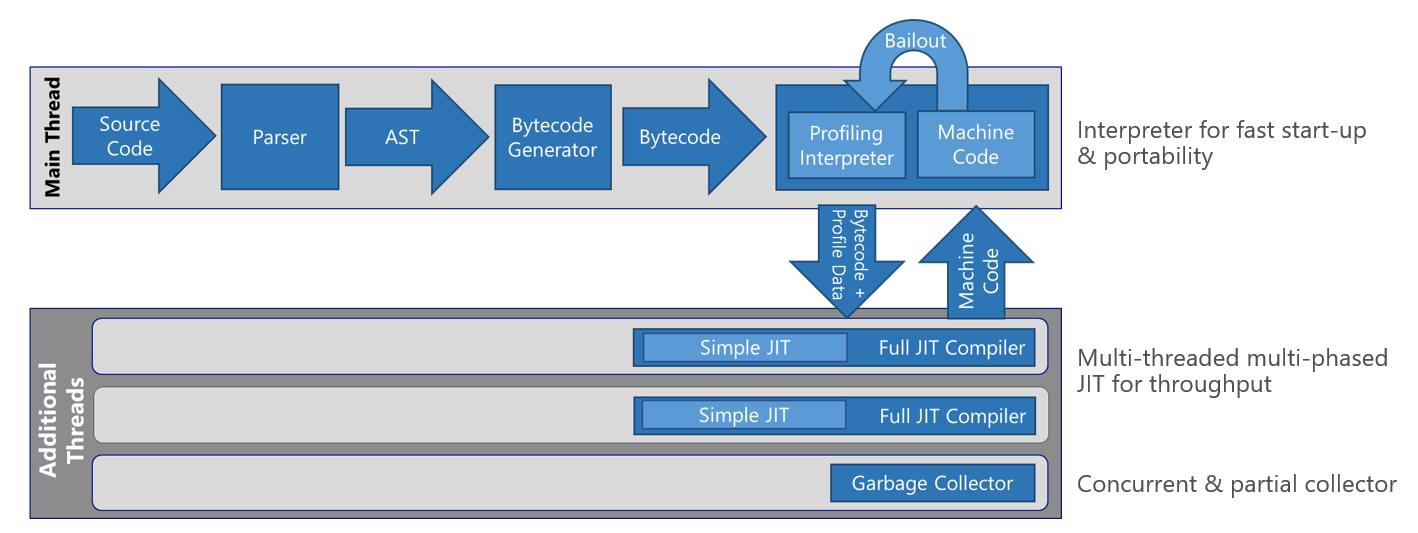
\includegraphics[width=14cm]{images/image-1}}
    }{
    \Fonte{\citeauthoronline{edgeengineopensource}}
    }
\end{figure}

Iniciando o processamento do código, como mostrado no esquema acima, será utilizado um
trecho de código que faz o cálculo do quadrado de um número e retorna o resultado desse
cálculo, como prova de conceito para mostrar passo a passo os resultados de cada etapa do
processo no motor \textit{JavaScript}. O trecho de código pode ser visto no Código-fonte
\ref{alg:code-1}.

\lstinputlisting[language=JavaScript,caption={\label{alg:code-1} \textit{Square} escrito em \textit{JavaScript}}]{code/square.js}

O motor ao receber o trecho de código inicia o \textit{parsing}, esse processo pode ser
dividido em dois subprocessos: Análise Léxica e Análise Sintática:

\begin{itemize}
    \item \textbf{Análise Léxica}: processo de quebrar uma entrada em uma sequência de
    símbolos (\textit{tokens}). \textit{Tokens} são o vocabulário linguístico: uma
    coleção de blocos de construção válidos, de acordo com uma gramática.
    \item \textbf{Análise Sintática}: processo de aplicação de regras de sintaxe, de
    acordo com uma gramática formal.
\end{itemize}

Cada um desses subprocessos possui um componente responsável por realizar tarefas
específicas de cada contexto, sendo eles:

\begin{itemize}
    \item \textbf{\textit{Lexer} ou \textit{Tokenizer}}: responsável por quebrar uma
    entrada em \textit{tokens} válidos, exercendo assim o papel de analisador léxico. O
    \textit{lexer} também sabe como tirar caminhos irrelevantes como espaços em branco e
    quebras de linha.
    \item \textbf{\textit{Parser}}: responsável pela construção da Árvore de Sintaxe
    Abstrata, em inglês \textit{Abtract Syntax Tree} (AST), analisando a estrutura do
    código de acordo com as regras de sintaxe da linguagem, buscando por possíveis erros
    baseado na escrita padrão da linguagem, para evitar erros durante a compilação ou
    resultados divergentes na execução do código ao final do processo.
\end{itemize}

O processo de \textit{parsing} é iterativo. O \textit{parser} solicita ao \textit{lexer}
um novo \textit{token}, e tenta combinar o \textit{token} recebido com uma das regras de
sintaxe. Se uma regra for correspondida, um novo nó correspondente ao \textit{token} é
adicionado a AST e o \textit{parser} solicitará o próximo \textit{token}, e assim
consecutivamente.

Se nenhuma regra corresponder, o \textit{parser} armazenará o \textit{token} internamente
e continuará pedindo \textit{tokens} até encontrar uma regra que corresponda a todos os
\textit{tokens} armazenados internamente. Se nenhuma regra for encontrada, que corresponda
aos \textit{tokens} armazenados, o \textit{parser} lançará uma exceção. Isso significa que o
código fornecido não é válido e possui erros de sintaxe.

Com base na função \textit{square} citada anteriormente, será obtido como resultado do
\textit{parsing} utilizando o primeiro subprocesso, \textit{tokenizer}
\footnote[1]{\textit{Tokenizer} pode ser compreendido como o processo de analisar uma
entrada de caracteres, como um código-fonte, e produzir uma sequência de símbolos que
podem ser manipulados mais facilmente por um \textit{parser}.}, os \textit{tokens} que
serão gerados e posteriormente analisados, cada um possuindo seu próprio tipo. Os
\textit{tokens} possem ser observados na Figura \ref{fig:image-2}.

\begin{figure}[h!]
    \centering
    \Caption{\label{fig:image-2} Resultado do \textit{Tokenizer} com base na função \textit{square}}
    \UECEfig{}{
    \fbox{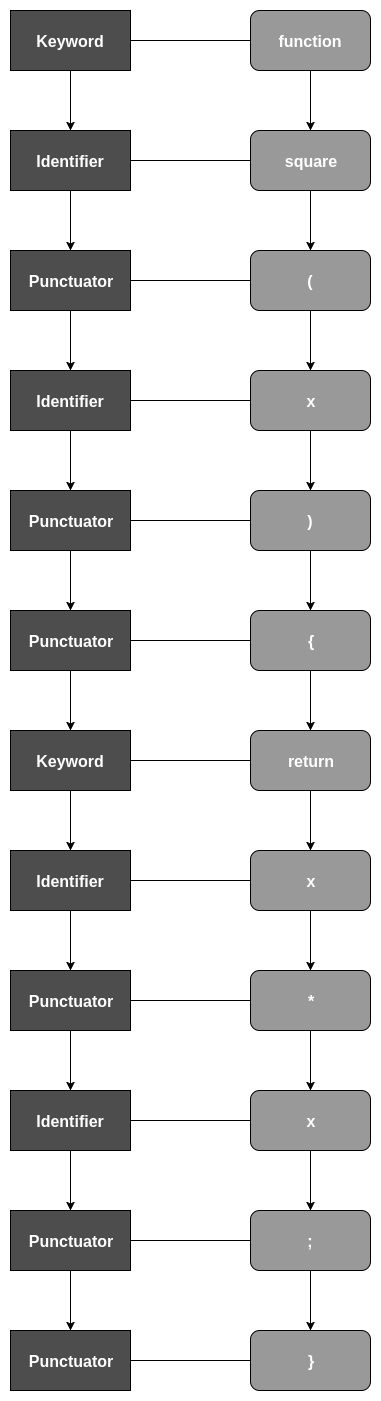
\includegraphics[width=4cm]{images/image-2}}
    }{
    \Fonte{Elaborada pelo autor.}
    }
\end{figure}

Após o resultado do \textit{tokenizer} ser gerado, uma Árvore de Sintaxe Abstrata, é
criada, para a função de potenciação conforme é mostrado na Figura \ref{fig:image-3}.

\begin{figure}[h!]
    \centering
    \Caption{\label{fig:image-3} Árvore de Sintaxe Abstrata gerada com base na função \textit{square}}
    \UECEfig{}{
    \fbox{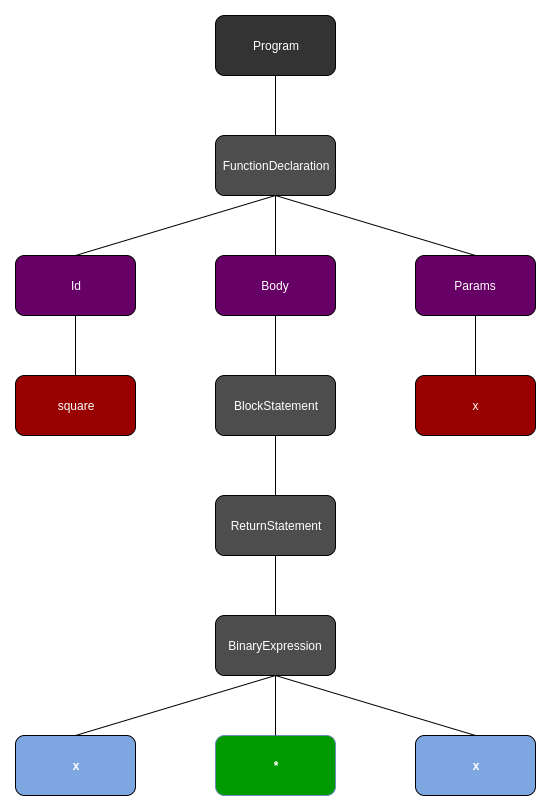
\includegraphics[width=8cm]{images/image-3}}
    }{
    \Fonte{Elaborada pelo autor.}
    }
\end{figure}

Após a geração da AST, com base na implementação do motor \textit{JavaScript}, o
\textit{bytecode generator} a converte para uma linguagem intermediária ou para código
nativo\footnote[2]{Conforme descrito acima, a etapa de geração do \textit{bytecode} pode
variar de acordo com a implementação do motor \textit{JavaScript}. Deixando a decisão de
utilizar ou não uma linguagem intermediária para o responsável pela implementação do
motor.}, e isso é feito para cada bloco de código representado na AST. Pode-se citar como
exemplo, alguns motores implementados até então:

\begin{itemize}
    \item \textbf{\textit{V8}}: implementado por um time da empresa Google e que é
    utilizado em seus navegadores, como \textit{Google Chrome} e \textit{Chromium}, que
    converte a AST diretamente para código nativo.
    \item \textbf{\textit{SpiderMonkey}}: o primeiro motor desenvolvido, criado pelo mesmo
    criador da linguagem \textit{JavaScript}, Brendan Eich, na Netscape e atualmente
    mantido pela Mozilla e que é utilizado em seus navegadores como
    \textit{Mozilla Firefox} e \textit{Firefox Nightly}, que converte a AST para uma
    linguagem intermediária.
    \item \textbf{\textit{Rhino}}: implementado e mantido por um time da empresa Mozilla,
    que por ser escrito utilizando a linguagem \textit{Java}, adiciona a etapa de tradução
    do código \textit{JavaScript} para classes \textit{Java}.
    \item \textbf{\textit{Chakra}}: implementado e mantido pela Microsoft, e que é
    utilizado no navegador \textit{Microsoft Edge}, que converte a AST para uma linguagem
    intermediária.
\end{itemize}

Códigos escritos em forma de \textit{bytecode} são formas canônicas de representação de
códigos que são utilizados pelos motores \textit{JavaScript}, são representações
intermediárias, que são projetadas para obter uma execução eficiente através de um
\textit{software} interpretador. Na Figura \ref{fig:image-4}, pode-se verificar o
\textit{bytecode} gerado, utilizando o motor \textit{SpiderMonkey}, para a função
\textit{square} utilizada como referência.

\begin{figure}[h!]
    \centering
    \Caption{\label{fig:image-4} Informações do \textit{bytecode} gerado com base na função \textit{square}}
    \UECEfig{}{
    \fbox{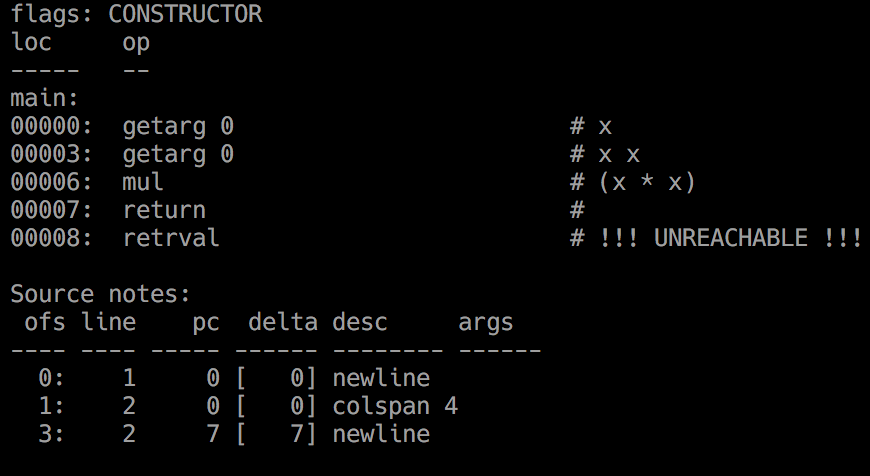
\includegraphics[width=10cm]{images/image-4}}
    }{
    \Fonte{Elaborada pelo autor.}
    \Nota{Informações obtidas utilizando a ferramenta \textit{JavaScript Shell} fornecida
    pelo motor \textit{SpiderMonkey}, usando internamente a função \textit{dis} da
    ferramenta.}
    }
\end{figure}

Após o \textit{bytecode} ter sido gerado, passa-se para a etapa de interpretação e
execução da representação intermediária, que é feita processando uma instrução por vez
percorrendo o \textit{bytecode} gerado. Quando o \textit{bytecode} chega até a área de
execução, observa-se a existência de dois componentes importantes para a performance de um
motor \textit{JavaScript}, que são o JIT (\textit{Just-in-Time Compiler}) e o Coletor de
Lixo (\textit{Garbage Collector}).

JIT, ou \textit{Just-in-Time compiler}, é o responsável por fazer a tradução de
\textit{bytecode} para código de máquina durante a execução do programa, ou seja, assim
que um trecho de código é solicitado, o JIT faz a transformação do \textit{bytecode} para
código de máquina, referente ao bloco solicitado e o disponibiliza para execução, fazendo
com que a disponibilização do resultado seja rápida e não consuma ciclos de processamento
desnecessários, entregando somente os blocos que serão utilizados no momento em que forem
solicitados.

O outro componente importante é o Coletor de Lixo, que é a área responsável pelo
gerenciamento automático da memória que é ocupada por objetos, sendo denominados como
"lixo" as posições de memória que estão sendo ocupadas com informações referentes ao
programa em execução, mas que não são relevantes ou que não estão sendo utilizadas.

Ambos os componentes comentados anteriormente, JIT e Coletor de Lixo, são executados
quando existe uma solicitação de um trecho de código \textit{JavaScript}, e estão
disponíveis durante toda a execução do motor \textit{JavaScript}, por isso estão
diretamente ligados ao passo de execução dentro do processo de interpretação de um código
\textit{JavaScript}.

Entretanto, no V8, que não utiliza uma representação intermediária, esse processo é um
pouco diferente. Ele utiliza dois compiladores, que podem ser denominados como o
compilador simples e o otimizador. O compilador simples é um compilador que não tem foco
em otimização, apesar de ainda assim realizar algumas, tem como principal objetivo
produzir código nativo tão rápido quanto possível, o que é importante para manter os
tempos de carregamento de uma página rápidos. \textit{Crankshaft}, e o atual
\textit{TurboFan}, são exemplos de compiladores com foco em otimização, também conhecidos
como otimizadores. O \textit{V8} compila todo o código com o compilador simples e em seguida
utiliza um \textit{profiler}\footnote[1]{\textit{Profiling} é uma forma de análise de
código dinâmica, que mede por exemplo, a complexidade espacial ou temporal de um algoritmo
específico, ou a frequência e duração de chamadas de funções. Comumente, um
\textit{profiler} serve para auxiliar a otimização de aplicações, selecionando quais
trechos de código darão um maior desempenho se otimizadas.} interno para selecionar as
funções a serem otimizadas, na maioria dos casos são as funções mais acessadas ou com
maior custo de processamento, pelo otimizador.

\section{\textit{WebAssembly}}
\label{sec:webassembly}

De acordo com a definição encontrada na especificação, ainda em desenvolvimento, do
\textit{WebAssembly}, é descrito que ele é um formato de código seguro, portátil e de
baixo nível projetado para uma execução eficiente e que possui uma representação compacta.
O objetivo principal é permitir que aplicações de alto desempenho sejam executados na
\textit{web}, mas não faz quaisquer pressupostos específicos da \textit{web} ou requer
quaisquer recursos específicos da \textit{web}, sendo assim pode ser empregado em outros
ambientes. \textit{WebAssembly} é um padrão aberto desenvolvido por um grupo comunitário
da W3C (\textit{World Wide Web Consortium})
\footnote[2]{\url{https://www.w3.org/community/webassembly/}} que inclui representantes de
todos os principais fornecedores de navegadores. A especificação descreve a versão 1.0 do
padrão central do \textit{WebAssembly}, e pretende-se que seja substituído por novos
lançamentos incrementais com recursos adicionais no futuro. \cite{wa}

\textit{WebAssembly} é a primeira solução para a execução de código de baixo nível na
\textit{web} que oferece todos os objetivos abaixo. É o resultado de uma colaboração sem
precedentes entre os principais fornecedores de navegadores e um grupo comunitário on-line
para construir uma solução comum para aplicativos de alto desempenho. \cite{wapaper}

Segundo a atual especificação, o \textit{WebAssembly} possui alguns objetivos principais
em sua modelagem:

\begin{itemize}
    \item Semântica rápida, segura e portátil:
    \begin{itemize}
        \item \textbf{Rápido}: execução com o desempenho próximo do código nativo,
        aproveitando as capacidades comuns a todos os \textit{hardwares} contemporâneos.
        \item \textbf{Seguro}: código validado e executado em um ambiente autocontido e
        seguro no que se refere a memória, impedindo a corrupção de dados ou violações de
        segurança.
        \item \textbf{Bem definido}: define de forma completa e precisa programas válidos
        e seu comportamento, de forma que seja fácil argumentar formalmente e/ou
        informalmente.
        \item \textbf{Independente de \textit{Hardware}}: código pode ser compilado em
        todas as arquiteturas modernas, dispositivos \textit{desktop} ou móveis e em
        sistemas integrados.
        \item \textbf{Independente de linguagem}: não privilegia nenhuma linguagem,
        modelo de programação ou modelo de objeto específico.
        \item \textbf{Independente de plataforma}: pode ser incorporado em navegadores,
        pode ser executado como uma VM autônoma ou integrado em outros ambientes.
        \item \textbf{Aberto}: programas podem interoperar com seu ambiente de forma
        simples e universal.
    \end{itemize}
    \item Representação eficiente e portátil:
    \begin{itemize}
        \item \textbf{Compacto}: possui um formato binário que é mais rápido de ser
        transmitido, sendo menor que os formatos de texto típicos ou os formatos de
        código nativo.
        \item \textbf{Modularizado}: aplicações podem ser divididas em partes menores que
        podem ser transmitidas, armazenadas em \textit{cache} e consumidas separadamente.
        \item \textbf{Eficiente}: pode ser decodificado, validado e compilado em uma única
        passagem rápida, igualmente como é feito com compilação \textit{just-in-time}
        (JIT) ou \textit{ahead-of-time} (AOT).
        \item \textbf{Fluido}: permite que os processos de decodificação, validação e
        compilação sejam iniciados o mais rápido possível, antes de todos os dados serem
        recebidos.
        \item \textbf{Paralelizável}: permite que os processos de decodificação, validação
        e compilação sejam divididos em muitas tarefas paralelas independentes.
        \item \textbf{Portável}: não faz nenhum pressuposto de arquitetura que não seja
        amplamente suportada por um \textit{hardware} moderno.
    \end{itemize}
\end{itemize}

Além disso, o \textit{WebAssembly} também se destina a ser fácil de inspecionar e depurar,
especialmente em ambientes como navegadores \textit{web}, mas esses recursos não serão
tratados na especificação atual. \cite{wa}

Antes de prosseguir, é necessário que se tenha conhecimento de alguns conceitos-chave
sobre \textit{WebAssembly}, pois serão necessários para entender seu fluxo de
processamento posteriormente:

\begin{itemize}
    \item \textbf{Módulo}: aplicações \textit{WebAssembly} são organizadas em módulos, que
    são a unidade básica de implantação, carregamento e compilação. Um módulo contém
    definições de tipos, funções, tabelas, memórias e variáveis globais. Além disso, pode
    declarar importações e exportações e fornecer lógica de inicialização na forma de
    segmentos de dados\footnote[1]{O conteúdo inicial de uma memória são \textit{bytes}
    "zero". O componente de dados de um módulo, \textit{data}, define um vetor de dados
    que inicializa um intervalo de memória em um determinado deslocamento com um vetor
    estático de \textit{bytes}.} e elementos\footnote[2]{O conteúdo inicial de uma tabela
    não está inicializada. O componente de elementos de um módulo, \textit{elem}, define
    um vetor de elementos que inicializa um intervalo de uma tabela em um determinado
    deslocamento com um vetor estático de elementos.} ou uma função de início.
    \item \textbf{Funções}: o código interno de um módulo é organizado em funções
    individuais. Cada função possui uma sequência de valores como parâmetros e retorna uma
    sequência de valores como resultado, conforme definido pelo seu tipo de função.
    \item \textbf{Instruções}: o processamento de um código \textit{WebAssembly} é baseado
    em uma máquina de pilha. O código de uma função consiste em uma sequência de
    instruções que manipulam valores em uma pilha de operandos implícita, desempilhando
    valores de argumentos e empilhando valores de resultados. No entanto, graças ao
    sistema de tipos, o leiaute da pilha de operandos pode ser determinado de forma
    estática em qualquer ponto do código, de modo que as implementações reais possam
    compilar o fluxo de dados entre as instruções diretamente sem nunca materializar a
    pilha de operandos. A organização da pilha é meramente uma maneira de conseguir uma
    representação compacta do programa, foi escolhido esse modelo pois se mostrou menor do
    que uma máquina registradora.
    \item \textbf{Memória}: o armazenamento principal de um módulo \textit{WebAssembly} é
    um grande vetor de \textit{bytes}, funcionando com uma memória linear. O tamanho do
    vetor sempre é um múltiplo do tamanho da página, páginas são subdivisões da memória
    para permitir-lhe uma utilização mais eficiente. Os \textit{bytes} podem ser
    manipulados através de instruções de memória, a execução de um segmento de dados, ou
    por meios externos fornecidos por quem está acoplando o \textit{WebAssembly}, um motor
    \textit{JavaScript} ou um sistema operacional por exemplo, que pode ser chamado de
    \textit{embedder}.
    \item \textbf{Exceções}: algumas instruções podem produzir um erro inesperado, que
    imediatamente aborta o processamento atual. As exceções atualmente não podem ser
    manipuladas por um código \textit{WebAssembly}, mas o \textit{embedder} normalmente
    fornecerá meios para lidar com essa condição. Se um código \textit{WebAssembly} for
    utilizado por um motor \textit{JavaScript} e ocorrer um erro interno, será lançada uma
    exceção \textit{JavaScript} contendo um \textit{stacktrace} com uma pilha de chamadas
    \textit{JavaScript} e \textit{WebAssembly}, que poderá ser manipulado por um código
    \textit{JavaScript}.
\end{itemize}

\subsection{Compilador}
\label{ssec:wa-compiler}

Quando se envia um código para ser executado na máquina de um usuário na \textit{web}, não
se sabe qual será a arquitetura de destino em que o código será executado. Então, o
\textit{WebAssembly} é um pouco diferente de outros tipos de \textit{assembly}. É um
idioma de máquina para uma máquina conceitual, e não para uma máquina física real, pode-se
dizer então que instruções \textit{WebAssembly} são instruções virtuais. Essas instruções
têm um mapeamento muito mais direto para o código de máquina do que o código-fonte
\textit{JavaScript}. Eles representam uma espécie de interseção do que pode ser feito de
forma eficiente em todo o \textit{hardware} popular comum, mas eles não são mapeamentos
diretos para o código de máquina específico de um \textit{hardware} específico. Pode-se
ver isso na Figura \ref{fig:image-5}.

\begin{figure}[h!]
    \centering
    \Caption{\label{fig:image-5} Processo de compilação de um código \textit{WebAssembly}}
    \UECEfig{}{
    \fbox{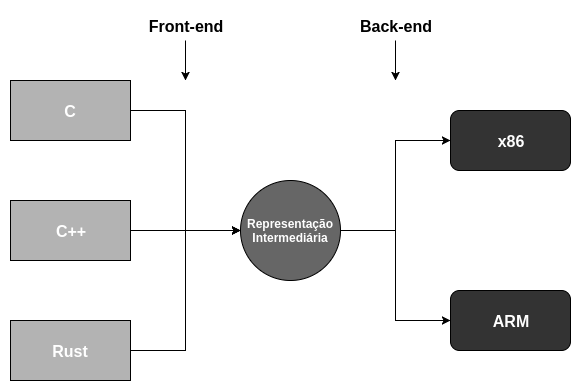
\includegraphics[width=10cm]{images/image-5}}
    }{
    \Fonte{Elaborada pelo autor.}
    }
\end{figure}

Até então, o projeto que possui maior suporte a \textit{WebAssembly} é o LLVM,
\textit{Low Level Virtual Machine}, que é uma infraestrutura de compilação, em que,
segundo Lattner, fornece componentes modulares e reutilizáveis para a construção de
compiladores, que auxiliam na redução de custo e tempo na criação de um compilador
particular. Essa infraestrutura possui uma representação intermediária própria, além
de diversas bibliotecas e componentes com interfaces bem definidas e ferramentas
construídas pelas próprias bibliotecas. LLVM fornece componentes totalmente independentes
de linguagem e máquina alvo, permitindo assim, que algoritmos de diferentes linguagens
possam ser conectados e otimizados em conjunto. \cite{llvm-intro}

LLVM é baseado na forma de atribuição única estática, em inglês
\textit{Static Single Assignment form} (SSA), que conforme Lattner e Adve, fornece
segurança de tipo, operações de baixo nível, flexibilidade e a capacidade de representar
todas as linguagens de alto nível de forma simples. A forma SSA é uma propriedade de uma
representação intermediária em que cada variável é atribuída exatamente uma vez, e cada
variável é definida antes de ser utilizada. \cite{llvm-langref}

Supondo que queira-se ir de \textit{C} para \textit{WebAssembly}, pode ser utilizado o
\textit{front-end} clang\footnote[1]{\url{https://clang.llvm.org}} para passar de
\textit{C} para a representação intermediária do LLVM. Uma vez que se está na RI do LLVM,
ele o entende, e então pode executar algumas otimizações. Para ir da RI do LLVM para o
\textit{WebAssembly}, é preciso um \textit{back-end}. Existe um que está atualmente em
andamento no projeto LLVM, e está com a sua maior parte implementada e deve ser finalizado
em breve. No entanto, ainda não é possível utilizá-lo. Existe outra ferramenta chamada
\textit{Emscripten}, que possui o seu próprio \textit{back-end} que pode produzir
\textit{WebAssembly} compilando para outra representação, denominada \textit{asm.js}, e em
seguida, convertendo-o para \textit{WebAssembly}. Pode-se ver isso na Figura
\ref{fig:image-6}.

\begin{figure}[h!]
    \centering
    \Caption{\label{fig:image-6} Ferramenta de compilação}
    \UECEfig{}{
    \fbox{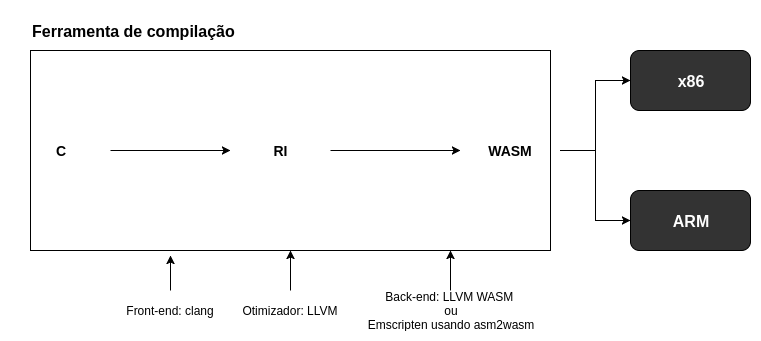
\includegraphics[width=12cm]{images/image-6}}
    }{
    \Fonte{Elaborada pelo autor.}
    }
\end{figure}

\subsection{Representação Intermediária}
\label{ssec:wa-ir}

Para permitir que o \textit{WebAssembly} seja lido e editado mais facilmente, existe uma
representação textual, além da representação binária (\textit{WASM}) citada anteriormente,
o \textit{WAST}. É um formato intermediário projetado para ser utilizado em editores de
texto, ferramentas de desenvolvimento, e até mesmo em navegadores.

Em ambos os formatos, binário e textual, a unidade fundamental de um código
\textit{WebAssembly} é um módulo. No formato de texto, um módulo é representado como uma
grande expressão em S. As expressões \textit{S} são um formato textual muito antigo e
muito simples para representar árvores, e assim pode-se pensar em um módulo como uma
árvore de nós que descrevem a estrutura do módulo e seu código. Ao contrário da árvore de
sintaxe abstrata de uma linguagem de programação, a árvore de um código
\textit{WebAssembly} é bastante plana, principalmente composta por listas de instruções.
Pode-se ver um exemplo no Código-fonte \ref{alg:code-2}.

\lstinputlisting[language=Lisp,caption={\label{alg:code-2} Exemplo de um módulo na representação intermediária textual}]{code/module.cl}

Todo o código em um módulo \textit{WebAssembly} é agrupado em funções, que possuem a
seguinte estrutura de pseudo-código:

\lstinputlisting[language=Lisp,caption={\label{alg:code-3} Estrutura de uma expressão \textit{S}}]{code/module-signature.cl}

\begin{itemize}
    \item \textbf{\textit{Signature}}: declara o que a função requer (parâmetros) e
    retorna (valores de retorno).
    \item \textbf{\textit{Locals}}: são definições de variáveis com tipos explícitos
    declarados.
    \item \textbf{\textit{Body}}: é apenas uma lista linear de instruções de baixo nível.
\end{itemize}

O formato textual também pode ser utilizado para simplificar a criação de um compilador
de uma linguagem específica para \textit{WebAssembly}, pois basta o novo compilador
suportar a representação textual e posteriormente utilizar um outro compilador que utilize
essa representação textual para a representação binária.

\subsection{Fluxo de processamento de um código \textit{WebAssembly}}
\label{ssec:wa-flow}

O esquema lógico apresentado na Figura \ref{fig:image-7} mostra o fluxo de processamento
de um código \textit{WebAssembly}, desde a compilação até sua execução, destacando as
etapas mais significativas para a explicação.

\begin{figure}[h!]
    \centering
    \Caption{\label{fig:image-7} Esquema lógico sequencial de processamento de um código \textit{WebAssembly}}
    \UECEfig{}{
    \fbox{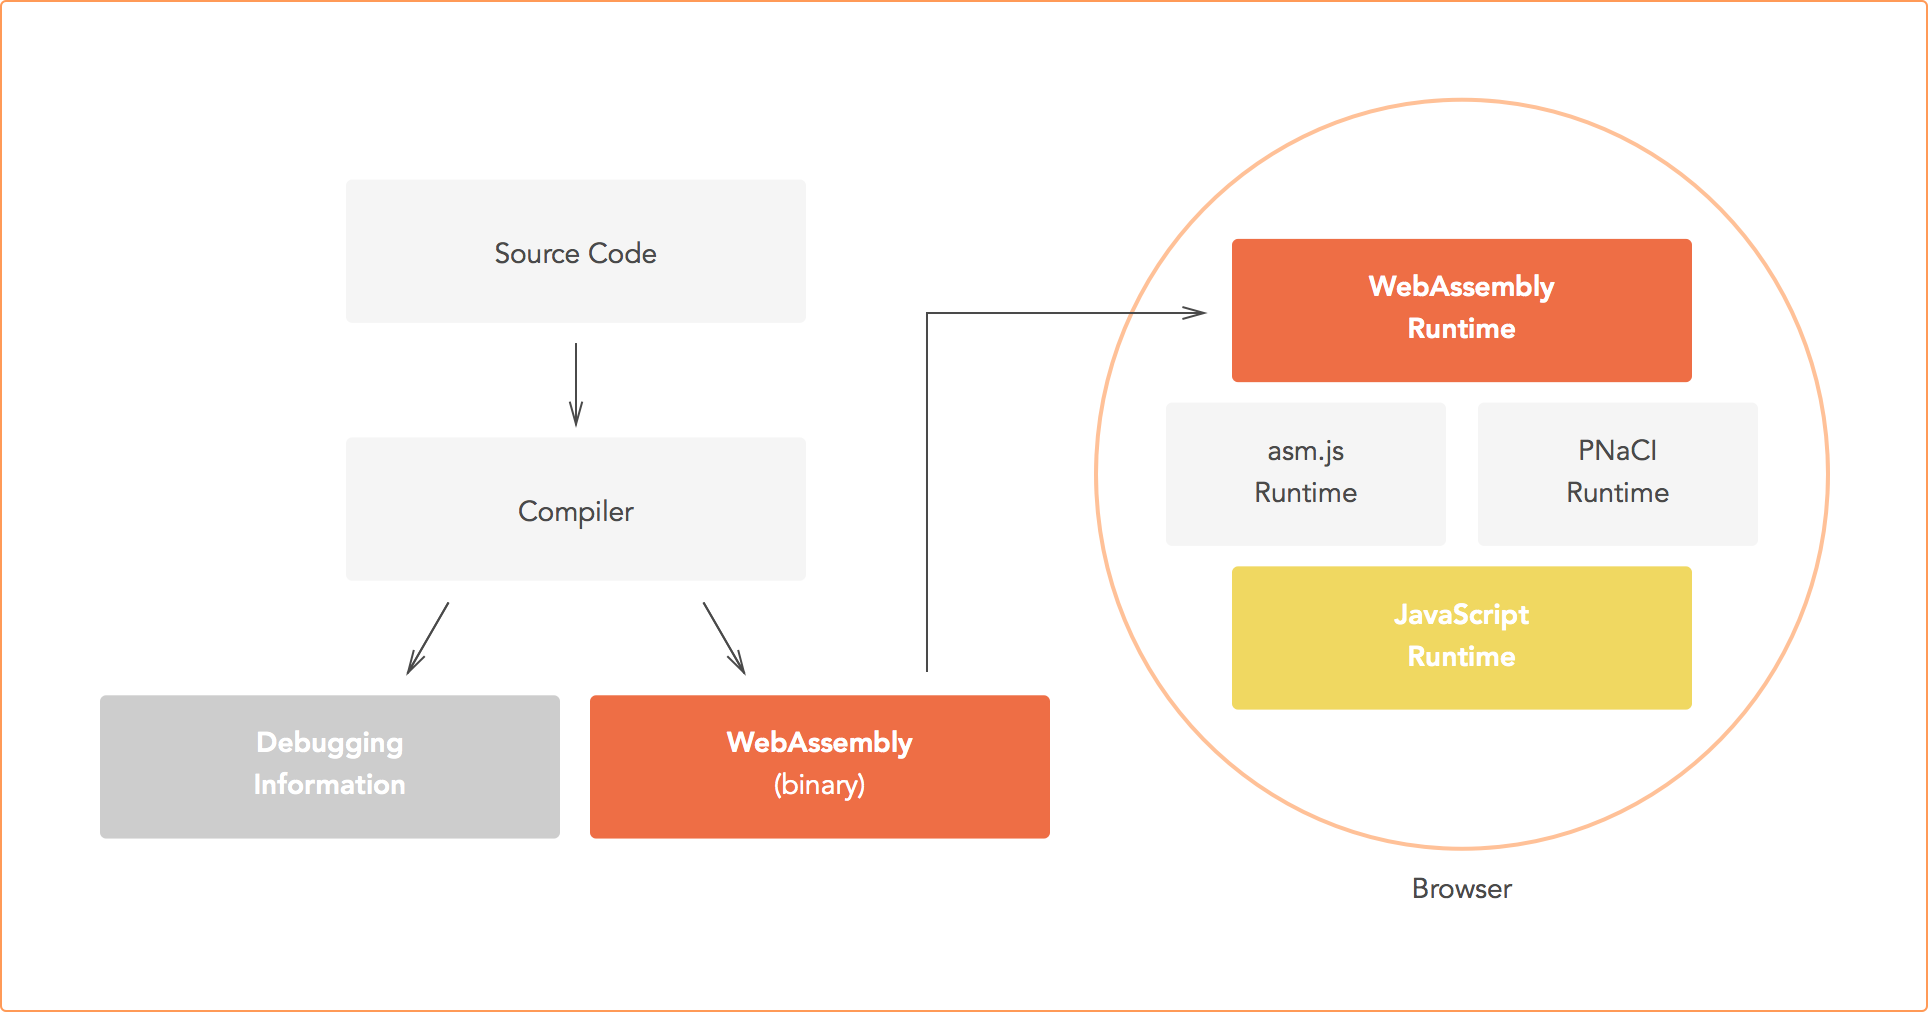
\includegraphics[width=12cm]{images/image-7}}
    }{
    \Fonte{\citeauthoronline{wa-things}}
    }
\end{figure}

Iniciando o processamento do código, conforme mostrado no esquema acima, será utilizada a
mesma função utilizada na seção anterior, alterando apenas a linguagem, \textit{C}, que
executa o cálculo do quadrado de um número e retorna o resultado desse cálculo, como prova
de conceito para mostrar passo a passo os resultados de cada etapa do processo realizado
pelo motor \textit{JavaScript}. O trecho de código pode ser visto no Código-fonte
\ref{alg:code-4}.

\lstinputlisting[language=C,caption={\label{alg:code-4} \textit{Square} escrito em \textit{C}}]{code/square.c}

Se for adicionado nesse processo a etapa de compilar a função \textit{square}, escrita em
\textit{C}, para a representação intermediária textual de \textit{WebAssembly}, serão
obtidos como saída as expressões \textit{S} exibidas na Figura \ref{fig:image-8}.

\begin{figure}[h!]
    \centering
    \Caption{\label{fig:image-8} Representação intermediária textual da função \textit{square}}
    \UECEfig{}{
    \fbox{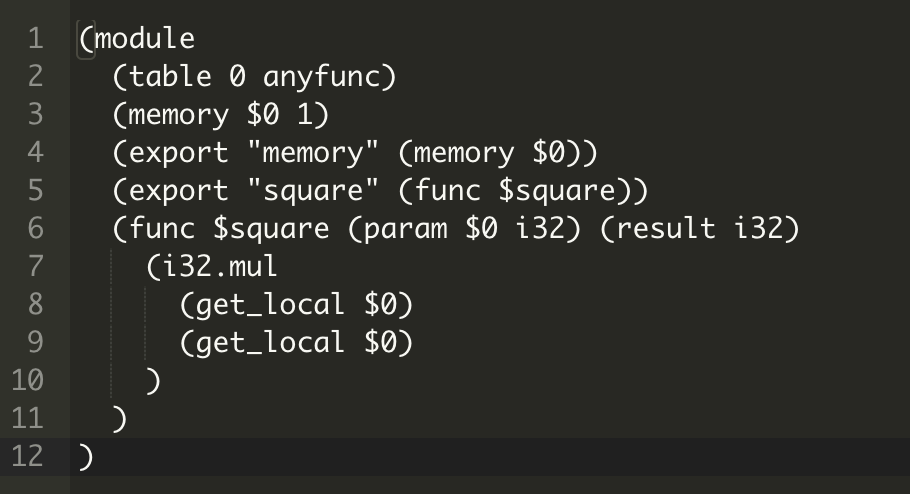
\includegraphics[width=12cm]{images/image-8}}
    }{
    \Fonte{Elaborada pelo autor.}
    \Nota{Expressões \textit{S} que representam a função \textit{square}.}
    }
\end{figure}

A próxima etapa é compilar da representação intermediária textual para a representação
intermediária binária, que é o formato que será utilizado durante a execução pelo motor
JavaScript. Pode-se observar a saída dessa etapa, onde é exibida a representação binária
da função \textit{square} na Figura \ref{fig:image-9}.

\begin{figure}[h!]
    \centering
    \Caption{\label{fig:image-9} Representação intermediária binária da função \textit{square}}
    \UECEfig{}{
    \fbox{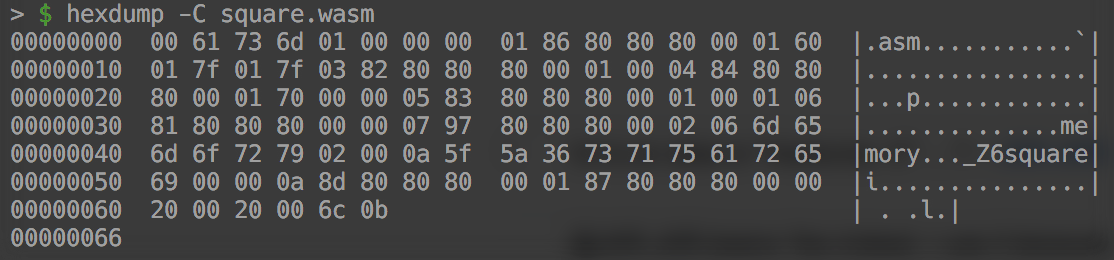
\includegraphics[width=14cm]{images/image-9}}
    }{
    \Fonte{Elaborada pelo autor.}
    \Nota{Imagem gerada utilizando a ferramenta \textit{hexdump} que exibe o conteúdo do
    arquivo utilizando notação hexadecimal.}
    }
\end{figure}

O último passo do processamento é carregar o módulo e executar a função \textit{square}.
Para isso será utilizado o código descrito no Código-fonte \ref{alg:code-5} que é
responsável por carregar, compilar e instânciar o módulo referente a essa função.

\lstinputlisting[language=JavaScript,caption={\label{alg:code-5} Carregamento e execução da função \textit{square}}]{code/load_module.js}

Na linha 1 é utilizada a função "fetch" fornecida pelo motor \textit{JavaScript} que
carrega o arquivo descrito, neste exemplo seria "square.wasm", e retorna um
\textit{promise} com o resultado. Na linha 2, é feita a leitura do conteúdo do arquivo e
é retornado um novo \textit{promise} com o conteúdo na forma de um vetor de
\textit{bytes}. Na linha 3, é utilizada a função \textit{instantiate} do objeto
\textit{WebAssembly} fornecida pelo motor \textit{JavaScript}, que compila o código
fornecido para código de máquina e retorna um objeto com dois campos, sendo o primeiro
campo o módulo representando o módulo \textit{WebAssembly} compilado e o segundo campo
sendo uma instância desse módulo que contém todas as funções exportadas por esse mesmo
módulo \textit{WebAssembly}. Vale ressaltar que nessa etapa podem ser lançadas exceções
caso ocorra algo inesperado durante a compilação, um exemplo disso pode ser
erros de tipo. Nas linhas 5 e 6, é utilizado o campo \textit{exports} da instância do
módulo que contém todas as funções exportadas e é executada a função \textit{square}.
Após o final da execução o valor 100 é exibido no \textit{console} do navegador, através
da função \textit{log} do objeto \textit{console} fornecida pelo motor
\textit{JavaScript}.
    \chapter{Desenvolvimento}
\label{chap:development}

Esta seção se dedica a descrever como realizar uma implementação utilizando
\textit{WebAssembly}. Para tanto, foi definida uma prova de conceito que consiste em uma
aplicação simples com a finalidade de mensurar a performance entre \textit{WebAssembly} e
\textit{JavaScript}, para que posteriormente seja possível realizar uma análise
comparativa entre os tempos de execução de algoritmos escritos em \textit{WebAssembly} e
\textit{JavaScript} utilizando o método \textit{StopWatch}.

Essa aplicação foi construída utilizando as três principais linguagens suportadas pelos
navegadores até então: \textit{HTML}, \textit{CSS} e \textit{JavaScript}. Entretanto para
a análise de desempenho foram construídos alguns algoritmos utilizando as linguagens
\textit{JavaScript} e \textit{C}, para que pudesse ser feita a comparação entre ambas as
execuções. Todos os testes foram realizados utilizando o navegador \textit{Google Chrome},
que utiliza o motor \textit{JavaScript V8}, e os algoritmos escritos em \textit{C} foram
compilados para a representação binária de \textit{WebAssembly} utilizando o compilador
\textit{Emscripten}.

Para a análise de desempenho foi utilizado o método \textit{StopWatch} que consiste em
medir o tempo decorrido entre o início e fim de uma tarefa. Para facilitar a compreensão
deste método, um exemplo de utilização desta técnica pode ser visto no Código-fonte
\ref{alg:code-6}.

\lstinputlisting[language=JavaScript,caption={\label{alg:code-6} Exemplo de utilização da técnica \textit{StopWatch}}]{code/stop_watch.js}

No código acima, pode-se ver que primeiro é obtido o tempo de início da tarefa antes de
executá-la, utilizando o método \textit{now} do objeto \textit{performance}, fornecido
pelo motor JavaScript, que retorna o tempo decorrido desde a criação do contexto de
uma página, em milissegundos. Logo em seguida, é executada a tarefa, através da função
\textit{task}, no exemplo citado. Posteriormente, é obtido o tempo final da tarefa,
utilizando novamente o método \textit{now} do objeto \textit{performance}, e logo depois,
é feita a subtração desses valores, obtendo então o tempo decorrido da execução da tarefa
em questão.

\section{Execução dos algoritmos}
\label{ssec:algorithms-execution}

Para a execução dos testes, foram selecionados 3 algoritmos, eles foram utilizados para
realizar uma análise simples sobre a execução de códigos escritos em \textit{JavaScript} e
\textit{WebAssembly}. São eles:

\begin{itemize}
    \item N-ésimo termo da sequência \textit{Fibonacci}
    \item \textit{ShellSort}
    \item \textit{QuickSort}
\end{itemize}

Para a execução dos algoritmos foram criados alguns objetos, com funções que simplificam
a manipulação dos algoritmos durante suas execuções. Entretanto, serão explicados mais
profundamente apenas os três principais objetos, selecionados devido sua importância
para a aplicação. Os objetos são:

\begin{itemize}
    \item \textit{Benchmark}
    \item \textit{Arrays}
    \item \textit{Runner}
\end{itemize}

O primeiro objeto, \textit{Benchmark}, foi o responsável por implementar a técnica
\textit{StopWatch} na aplicação, foi através dele que foi obtido o tempo decorrido de cada
algoritmo executado. Entretanto, ele não se limita apenas ao tempo de execução, sendo
responsável também por informar o resultado de cada algoritmo. A implementação desse
objeto pode ser vista no Código-fonte \ref{alg:code-7}.

\lstinputlisting[language=JavaScript,caption={\label{alg:code-7} Objeto \textit{Benchmark} utilizado na execução dos testes}]{code/benchmark.js}

O objeto \textit{Benchmark}, possui apenas uma única função, que recebe como parâmetro
o algoritmo a ser executado e retorna dois valores: o tempo decorrido e o resultado dessa
tarefa.

O segundo objeto, \textit{Arrays}, foi utilizado para realizar uma validação simples no
resultado de cada algoritmo: verificar se o resultado obtido através da implementação
em \textit{JavaScript} e \textit{WebAssembly} foi o mesmo. Esse objeto fazendo apenas
essa checagem, foi responsável por verificar quaisquer falha de manipulação de memória
que pudesse nos retornar um resultado falso positivo. A implementação desse objeto pode
ser vista no Código-fonte \ref{alg:code-8}.

\lstinputlisting[language=JavaScript,caption={\label{alg:code-8} Objeto \textit{Arrays} utilizado na execução dos testes}]{code/arrays.js}

O objeto \textit{Arrays} possui apenas uma única função, assim como o objeto
\textit{Benchmark}, que aceita dois vetores como parâmetro e retorna um valor do tipo
\textit{Boolean}, informando se os dois vetores possuem os mesmo valores ou não.

Da linha 2 a linha 4 são realizadas as validações mais simples, onde é verificado se um
dos dois vetores não possui valor, sendo retornado o valor verdadeiro em caso positivo e
falso em caso negativo. Como \textit{JavaScript} possui avaliação de curto-circuito, em
que os argumentos posteriores são avaliados apenas se os argumentos anteriores não forem
suficientes para determinar o valor da expressão, caso seja informado algum vetor vazio,
por exemplo, o motor já identificará nas primeiras condições que os vetores são
diferentes. Na linha 5, é verificado se o tamanho desses vetores é diferente, pois caso
sejam, os vetores em si já serão identificados como diferentes pois não possuem o mesmo
número de elementos. Na linha 6, é utilizado o método \textit{some} para checar elemento
por elemento de ambos os vetores, caso seja identificado em algum índice que os elementos
dos vetores são diferentes a iteração irá parar e será retornado o valor verdadeiro, caso
contrário será retornado o valor falso.

O terceiro objeto, \textit{Runner}, foi o responsável por implementar todo o fluxo de
execução dos algoritmos, manipulando memória quando necessário, gerando os vetores
iniciais que foram utilizados pelos algoritmos de ordenação, verificando o resultado de
cada algoritmo e calculando a relação entre o tempo decorrido entre os algoritmos
implementados em \textit{WebAssembly} e em \textit{JavaScript}. A implementação desse
objeto pode ser vista no Código-fonte \ref{alg:code-9}.

\lstinputlisting[language=JavaScript,caption={\label{alg:code-9} Objeto \textit{Runner} utilizado na execução dos testes}]{code/test_runner.js}

O objeto \textit{Runner} diferente dos dois objetos anteriores, possui três métodos, cada
um responsável pela execução de um algoritmo específico. Dada a importância da compreensão
desses métodos, serão explicados cada um deles individualmente a seguir.

Em cada uma das funções de execução, os parâmetros representam os mesmos objetos,
alterando apenas seus significados de acordo com o algoritmo analisado.

O primeiro parâmetro representa um objeto simples que possui três atributos:

\begin{itemize}
    \item \textit{\textbf{module}}: um objeto que representa a instância do módulo
    \textit{WebAssembly} relacionado ao algoritmo em questão.
    \item \textit{\textbf{wasm}}: uma função escrita em \textit{WebAssembly} relacionada
    ao algoritmo a ser analisado.
    \item \textit{\textbf{js}}: uma função escrita em \textit{JavaScript} relacionada ao
    algoritmo a ser analisado.
\end{itemize}

O segundo parâmetro representa um valor numérico, tendo significados distintos de acordo
com a função de execução.

Esta seção se dedica apenas a explicar a execução de cada um dos algoritmos propostos, e
não os próprios algoritmos em si, com a finalidade de fornecer todos os detalhes sobre
toda a manipulação necessária para a execução dos mesmos, mais detalhes de implementação
de cada uma das duas abordagens, \textit{JavaScript} e \textit{WebAssembly}, serão
explicados e analisados na próxima seção.

\lstinputlisting[language=JavaScript,caption={\label{alg:code-10} Função de execução do algoritmo \textit{Fibonacci}}]{code/fibonacci_test.js}

Iniciando a execução do primeiro algoritmo, seu objetivo é encontrar o n-ésimo termo da
sequência \textit{fibonacci}, sendo o termo a ser encontrado representado pelo segundo
parâmetro da função.

Analisando o código descrito no Código-fonte \ref{alg:code-10}, pode-se ver que nas
linhas 2 e 3, são executados ambos os algoritmos, utilizando o objeto \textit{Benchmark}
já mencionado anteriormente, em que são obtidos os seus resultados e tempos de execução.
Na linha 5 é verificado se os resultados obtidos são diferentes, retornando um valor nulo
caso essa regra seja obedecida, caso contrário a execução do método continua. Na linha 10,
é calculada a relação entre os tempos de execução entre os algoritmos escritos em
\textit{JavaScript} e \textit{WebAssembly}. Na linha 11, são retornados os valores obtidos
de ambas as execuções.

\lstinputlisting[language=JavaScript,caption={\label{alg:code-11} Função de execução do algoritmo \textit{ShellSort}}]{code/shellsort_test.js}

\textit{ShellSort} é um algoritmo de ordenação, de complexidade quadrática, que na
aplicação citada anteriormente, tem como objetivo colocar os elementos dos vetores em
ordem ascendente, ou seja, do elemento de menor valor para o de maior valor, sendo o
tamanho do vetor representado pelo segundo parâmetro da função.

Analisando o código descrito no Código-fonte \ref{alg:code-11}, pode-se ver que da linha 2
a linha 7 são gerados dois vetores de mesmo tamanho e mesmo valores, que serão utilizados
posteriormente. Na linha 9, foi criada uma variável representando a quantidade de
\textit{bytes} ocupados por um tipo flutuante, em \textit{WebAssembly} tipos flutuantes
podem ser de 32 ou 64 \textit{bits}, e como no algoritmo escrito em \textit{C} foi
utilizado o tipo \textit{double}, que em \textit{C} representa 64 \textit{bits}, quando
for gerada a representação binária do algoritmo, utilizando o \textit{Emscripten}, essas
mesmas variáveis de tipo \textit{double} serão representadas com 64 \textit{bits} em
\textit{WebAssembly}, por isso foi atribuído o valor 8 a essa variável representando os 8
\textit{bytes}. Na linha 10, foi criada uma variável para conter o último índice desses
vetores, que será utilizado posteriormente. Na linha 11, é utilizado o método
\textit{\_malloc} para alocar a memória necessária para os elementos do vetor "a" que será
passado para o código \textit{WebAssembly} posteriormente, ocupando 8 \textit{bytes}
por elemento do vetor. Na linha 12, é criada uma variável responsável por conter a
quantidade de deslocamento de \textit{bytes}, de acordo com a quantidade de \textit{bytes}
por elemento do vetor. Na linha 14, é utilizado o campo \textit{HEAPF64} que representa a
\textit{heap} responsável por armazenar campos flutuantes de 64 \textit{bits}. Abaixo
segue uma tabela de mapeamento, de que \textit{heap} utilizar com base em que tipo de
dado:

\begin{table}[ht]
    \Caption{\label{tab:heap} Tabela de mapeamento de \textit{Heap} para o tipo específico}
    \IBGEtab{}{
    \begin{tabular}{ccc}
        \toprule
        Heap & C++ & JavaScript \\
        \midrule \midrule
        HEAP8 & int8\_t & Int8Array \\
        HEAPU8 & uint8\_t & Uint8Array \\
        HEAP16 & int16\_t & Int16Array \\
        HEAPU16 & uint16\_t & Uint16Array \\
        HEAP32 & int32\_t & Int32Array \\
        HEAPU32 & uint32\_t & Uint32Array \\
        HEAPF32 & float & Float32Array \\
        HEAPF64 & double & Float64Array \\
    \end{tabular}
    }{
    \Fonte{Elaborado pelo autor.}
    }
\end{table}

Conforme explicado anteriormente, \textit{WebAssembly} utiliza uma memória linear, que
pode ser entendida como um simples vetor de elementos. Na tabela acima, pode-se ver que
tipo de vetor é utilizado em \textit{JavaScript} na implementação do \textit{WebAssembly}
para armazenar que tipo de dados. Até o momento, cada tipo de dado possui sua própria
\textit{heap}.

Continuando na linha 14, os dados são copiados do vetor para a \textit{heap}, de forma
que o código \textit{WebAssembly} possa manipulá-lo. Na linha 15, é executada a função em
\textit{WebAssembly} referente ao algoritmo \textit{ShellSort}, passando como parâmetro
para a função, a variável representando um ponteiro para o vetor, e o tamanho do vetor.
Na linha 16, são obtidos os valores que estão na \textit{heap} e são atribuídos de volta
ao vetor "a". Na linha 17, é removido da memória o espaço alocado anteriormente, dado
que não será utilizado posteriormente.

\lstinputlisting[language=JavaScript,caption={\label{alg:code-12} Função de execução do algoritmo \textit{QuickSort}}]{code/quicksort_test.js}

A implementação da função de execução do algoritmo \textit{QuickSort} é semelhante a
função do \textit{ShellSort}, tendo como única diferença os parâmetros que são passados
para as implementações dos algoritmos, enquanto no \textit{ShellSort} são passados apenas
dois parâmetros, que são o ponteiro para o vetor e o tamanho do vetor, no
\textit{QuickSort} são passados três parâmetros: o ponteiro representando o vetor, o
índice inicial do vetor e o índice final do vetor.

\section{Comparação}
\label{ssec:comparison}

Como descrito na seção anterior, foram selecionados 3 algoritmos para a realização da
análise do tempo de execução, sendo estes escritos nas linguagens \textit{JavaScript} e
\textit{C}:

\begin{itemize}
    \item N-ésimo termo da sequência \textit{Fibonacci}
    \item \textit{ShellSort}
    \item \textit{QuickSort}
\end{itemize}

A análise consiste da implementação desses algoritmos em cada linguagem, para a obtenção
do tempo de execução de cada um individualmente, utilizando a técnica \textit{StopWatch},
alterando apenas os dados de entrada. Todos os testes foram realizados utilizando o
navegador \textit{Google Chrome}, que utiliza o motor \textit{JavaScript V8}, e os
algoritmos escritos em \textit{C} foram compilados para a representação binária de
\textit{WebAssembly} utilizando a ferramenta \textit{Emscripten}.

O primeiro algoritmo a ser analisado foi o responsável por calcular o n-ésimo termo da
sequência \textit{Fibonacci}, para tanto foi utilizada a implementação em
\textit{JavaScript} que pode ser vista no Código-fonte \ref{alg:code-13}.

\lstinputlisting[language=JavaScript,caption={\label{alg:code-13} Algoritmo responsável por calcular o n-ésimo termo da sequência \textit{Fibonacci} em \textit{JavaScript}}]{code/fibonacci.js}

O mesmo algoritmo foi implementado em \textit{C} utilizando recursão e pode ser visto no
Código-fonte \ref{alg:code-14}.

\lstinputlisting[language=C,caption={\label{alg:code-14} Algoritmo responsável por calcular o n-ésimo termo da sequência \textit{Fibonacci} em \textit{C}}]{code/fibonacci.c}

Como foi possível observar nas implementações exibidas nos códigos-fonte \ref{alg:code-13}
e \ref{alg:code-14}, o mesmo algoritmo foi implementado em \textit{JavaScript} e em
\textit{C}, fazendo com que fosse possível obter o tempo decorrido de cada execução
isoladamente. Os tempos obtidos para cada implementação com base no termo a ser
encontrado, pode ser visto na Tabela \ref{tab:time-1}.

\begin{table}[ht]
    \Caption{\label{tab:time-1} Tempos de execução do algoritmo que calcula o n-ésimo termo da sequência \textit{Fibonacci}}
    \IBGEtab{}{
    \begin{tabular}{cccc}
        \toprule
        Termo & JavaScript (ms) & WebAssembly (ms) & Razão (JS / WA) \\
        \midrule \midrule
        5  & 0.11500     & 0.05500    & 2.09091 \\
        10 & 0.01500     & 0.02000    & 0.75000 \\
        15 & 0.16000     & 0.01000    & 16.00000 \\
        20 & 1.20000     & 0.05000    & 24.00000 \\
        25 & 0.82000     & 0.36500    & 2.24658 \\
        30 & 8.63500     & 3.13500    & 2.75439 \\
        35 & 94.79500    & 32.33500   & 2.93165 \\
        40 & 1098.46000  & 360.71000  & 3.04527 \\
        45 & 11907.52500 & 4212.73500 & 2.82655 \\
        \bottomrule
    \end{tabular}
    }{
    \Fonte{Elaborado pelo autor.}
    \Nota[Ambiente]{Teste realizado no navegador \textit{Google Chrome} que utiliza o motor
    \textit{JavaScript V8}.}
    }
\end{table}

Como foi possível perceber, com base na Tabela \ref{tab:time-1}, \textit{WebAssembly} se
mostrou mais eficiente que \textit{JavaScript} em quase todos os casos, com exceção da
execução do algoritmo que busca pelo décimo termo da sequência \textit{Fibonacci}, em que
a execução de \textit{JavaScript} foi de aproximadamente 30\% mais eficiente que a
execução em \textit{WebAssembly}, entretanto, no melhor caso, \textit{WebAssembly}
utilizou apenas aproximadamente 4\% do tempo decorrido pelo mesmo algoritmo escrito em
\textit{JavaScript}, onde buscou-se pelo vigésimo termo da sequência.

O segundo algoritmo trata-se de um algoritmo de ordenação denominado \textit{ShellSort},
que na aplicação proposta tem como objetivo colocar os elementos de um vetor em ordem
ascendente. A implementação feita em \textit{JavaScript} pode ser vista no
Código-fonte \ref{alg:code-15}.

\lstinputlisting[language=JavaScript,caption={\label{alg:code-15} \textit{ShellSort} em \textit{JavaScript}}]{code/shell_sort.js}

A mesma implementação do algoritmo \textit{ShellSort} foi realizada em \textit{C}, e pode
ser visto no Código-fonte \ref{alg:code-16}.

\lstinputlisting[language=C,caption={\label{alg:code-16} \textit{ShellSort} em \textit{C}}]{code/shell_sort.c}

O mesmo algoritmo foi implementado em \textit{JavaScript} e em \textit{C}, e foram obtidos
os seguintes resultados referentes ao tempo de execução e dados de entrada:

\begin{table}[ht]
    \Caption{\label{tab:time-2} Tempos de execução do algoritmo \textit{ShellSort}}
    \IBGEtab{}{
    \begin{tabular}{cccc}
        \toprule
        Tamanho do vetor & JavaScript (ms) & WebAssembly (ms) & Razão (JS / WA) \\
        \midrule \midrule
        10    & 0.10500  & 0.10500 & 1.00000 \\
        100   & 0.06500  & 0.01000 & 6.50000 \\
        1000  & 3.64500  & 0.09500 & 38.36842 \\
        2000  & 1.88500  & 0.20500 & 9.19512 \\
        3000  & 0.38000  & 0.31500 & 1.20635 \\
        4000  & 0.52000  & 0.47000 & 1.10638 \\
        5000  & 0.82000  & 0.67000 & 1.22388 \\
        25000 & 5.00500  & 4.09500 & 1.22222 \\
        50000 & 10.26000 & 8.42000 & 1.21853 \\
        \bottomrule
    \end{tabular}
    }{
    \Fonte{Elaborado pelo autor.}
    \Nota[Vetor]{Itens do vetor gerados aleatoriamente.}
    \Nota[Ambiente]{Teste realizado no navegador \textit{Google Chrome} que utiliza o
    motor \textit{JavaScript V8}.}
    }
\end{table}

Com base na Tabela \ref{tab:time-2}, pode-se observar que a execução do algoritmo escrito
em \textit{WebAssembly} teve performance superior ao escrito em \textit{JavaScript} em
quase todos os casos. No pior caso, o algoritmo em \textit{WebAssembly} utilizou
aproximadamente o mesmo tempo decorrido pelo algoritmo em \textit{JavaScript}, entretanto,
no melhor caso, o algoritmo escrito em \textit{WebAssembly} chegou a utilizar apenas
aproximadamente 3\% do tempo utilizado pelo algoritmo em \textit{JavaScript}, em que foi
utilizado um vetor com 1000 elementos.

O terceiro algoritmo também trata-se de um algoritmo de ordenação, denominado
\textit{QuickSort}, que na aplicação proposta tem como objetivo colocar os elementos de um
vetor em ordem ascendente. A implementação feita em \textit{JavaScript} pode ser vista no
Código-fonte \ref{alg:code-17}.

\lstinputlisting[language=JavaScript,caption={\label{alg:code-17} \textit{QuickSort} em \textit{JavaScript}}]{code/quick_sort.js}

O mesmo algoritmo foi implementado em \textit{C} e pode ser visto no Código-fonte
\ref{alg:code-18}.

\lstinputlisting[language=C,caption={\label{alg:code-18} \textit{QuickSort} em \textit{C}}]{code/quick_sort.c}

O mesmo algoritmo foi implementado em \textit{JavaScript} e em \textit{C}, e foram obtidos
os seguintes resultados referentes ao tempo de execução e dados de entrada:

\begin{table}[ht]
    \Caption{\label{tab:time-3} Tempos de execução do algoritmo \textit{QuickSort}}
    \IBGEtab{}{
    \begin{tabular}{cccc}
        \toprule
        Tamanho do vetor & JavaScript (ms) & WebAssembly (ms) & Razão (JS / WA) \\
        \midrule \midrule
        10       & 0.27000     & 0.06500    & 4.15385 \\
        100      & 0.07500     & 0.01000    & 7.50000 \\
        1000     & 2.37500     & 0.09000    & 26.38889 \\
        10000    & 1.23500     & 1.06500    & 1.15962 \\
        100000   & 15.78000    & 13.14000   & 1.20091 \\
        1000000  & 179.01000   & 160.65500  & 1.11425 \\
        10000000 & 2171.02000  & 1861.00500 & 1.16658 \\
        20000000 & 4224.75500  & 3724.26000 & 1.13439 \\
        30000000 & 6662.29500  & 5761.54500 & 1.15634 \\
        40000000 & 9594.70000  & 7917.12000 & 1.21189 \\
        50000000 & 11478.08000 & 9998.39500 & 1.14799 \\
        \bottomrule
    \end{tabular}
    }{
    \Fonte{Elaborado pelo autor.}
    \Nota[Vetor]{Itens do vetor gerados aleatoriamente.}
    \Nota[Ambiente]{Teste realizado no navegador \textit{Google Chrome} que utiliza o
    motor \textit{JavaScript V8}.}
    }
\end{table}

Analisando a Tabela \ref{tab:time-3}, pode-se observar que o algoritmo escrito em
\textit{WebAssembly} teve tempo de execução superior ao escrito em \textit{JavaScript} em
todos os casos, em que na melhor execução utilizou apenas aproximadamente 4\% do tempo
utilizado pelo mesmo algoritmo escrito em \textit{JavaScript}, onde foi utilizado um
vetor com 1000 elementos.

Com base nos resultados obtidos exibidos nas tabelas \ref{tab:time-1}, \ref{tab:time-2} e
\ref{tab:time-3}, foram gerados os gráficos exibidos nas figuras \ref{fig:image-10},
\ref{fig:image-11} e \ref{fig:image-12}. Esses gráficos possuem 4 dados-chave: os dados
de entrada, o tempo utilizado por ambas as implementações para conclusão da tarefa
proposta e a média de tempo gasto com base nos tempos de execução obtidos.

\begin{figure}[h!]
    \centering
    \Caption{\label{fig:image-10} Resultados do algoritmo que descobre o n-ésimo termo da sequência \textit{Fibonacci}}
    \UECEfig{}{
    \fbox{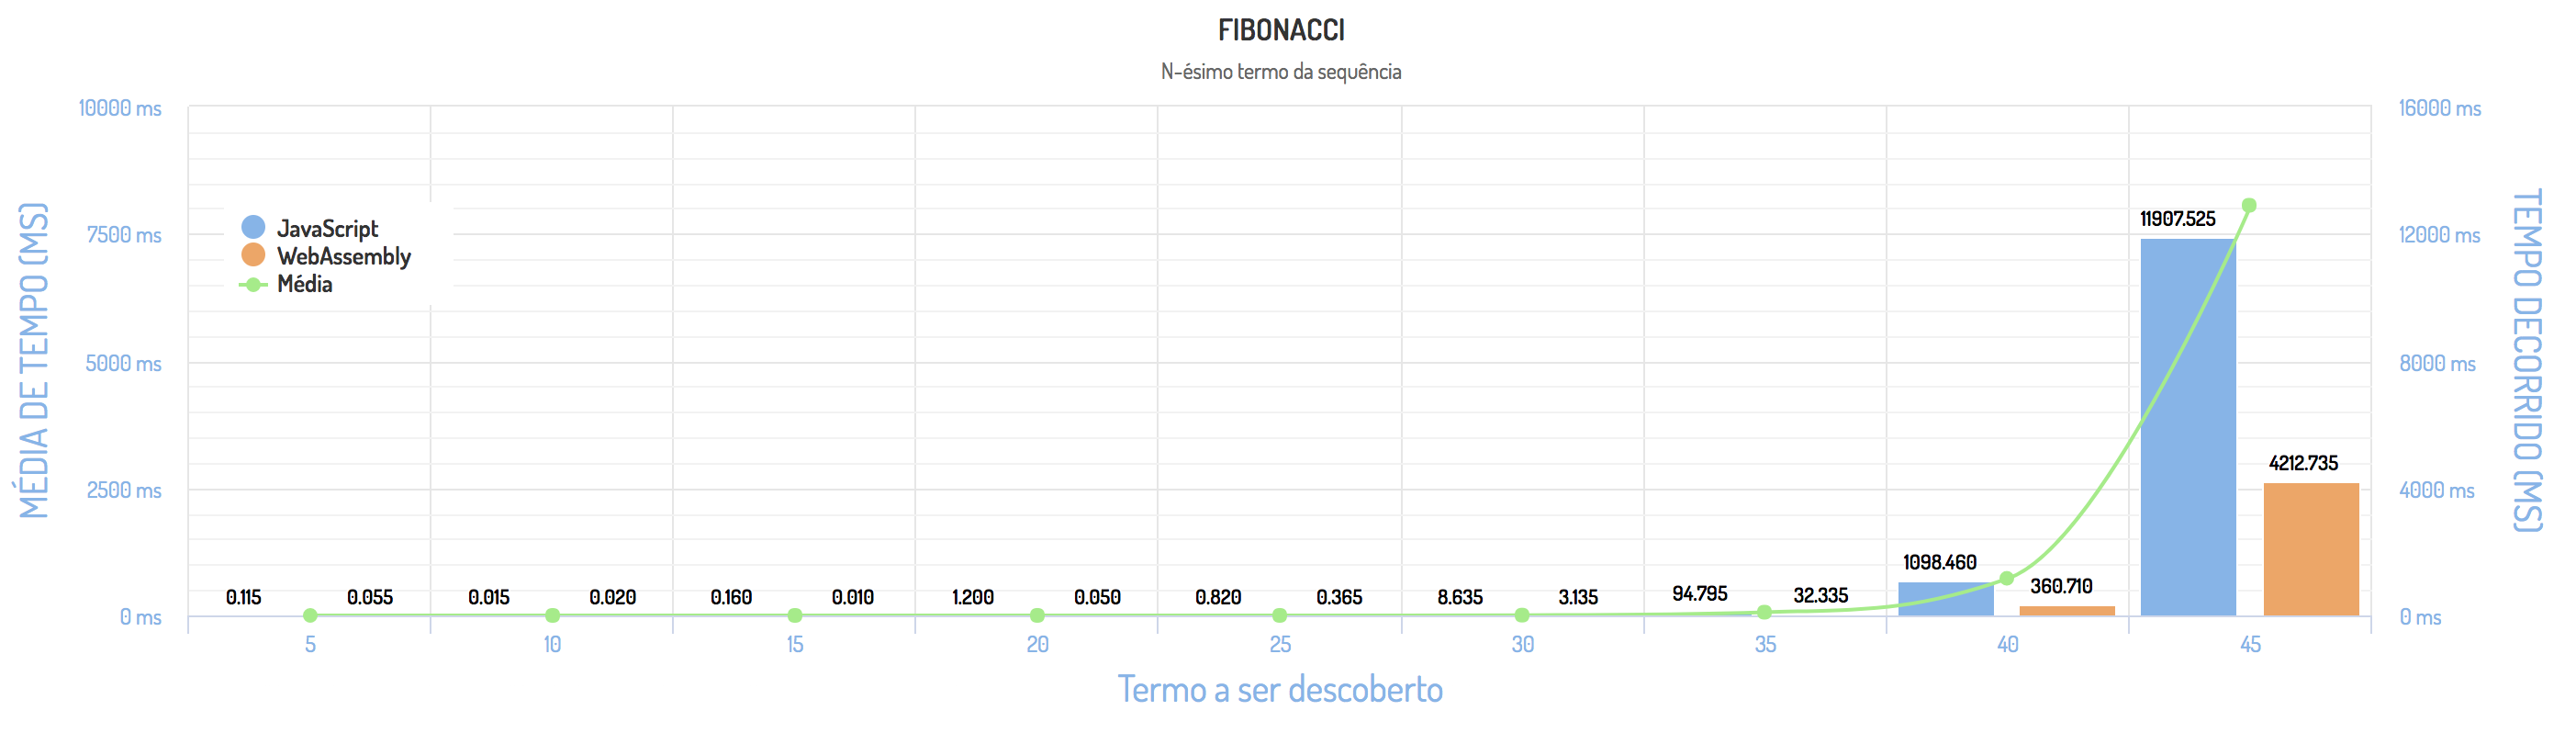
\includegraphics[width=16cm]{graphics/fibonacci}}
    }{
    \Fonte{Elaborada pelo autor.}
    }
\end{figure}

\begin{figure}[h!]
    \centering
    \Caption{\label{fig:image-11} Resultados do algoritmo \textit{ShellSort}}
    \UECEfig{}{
    \fbox{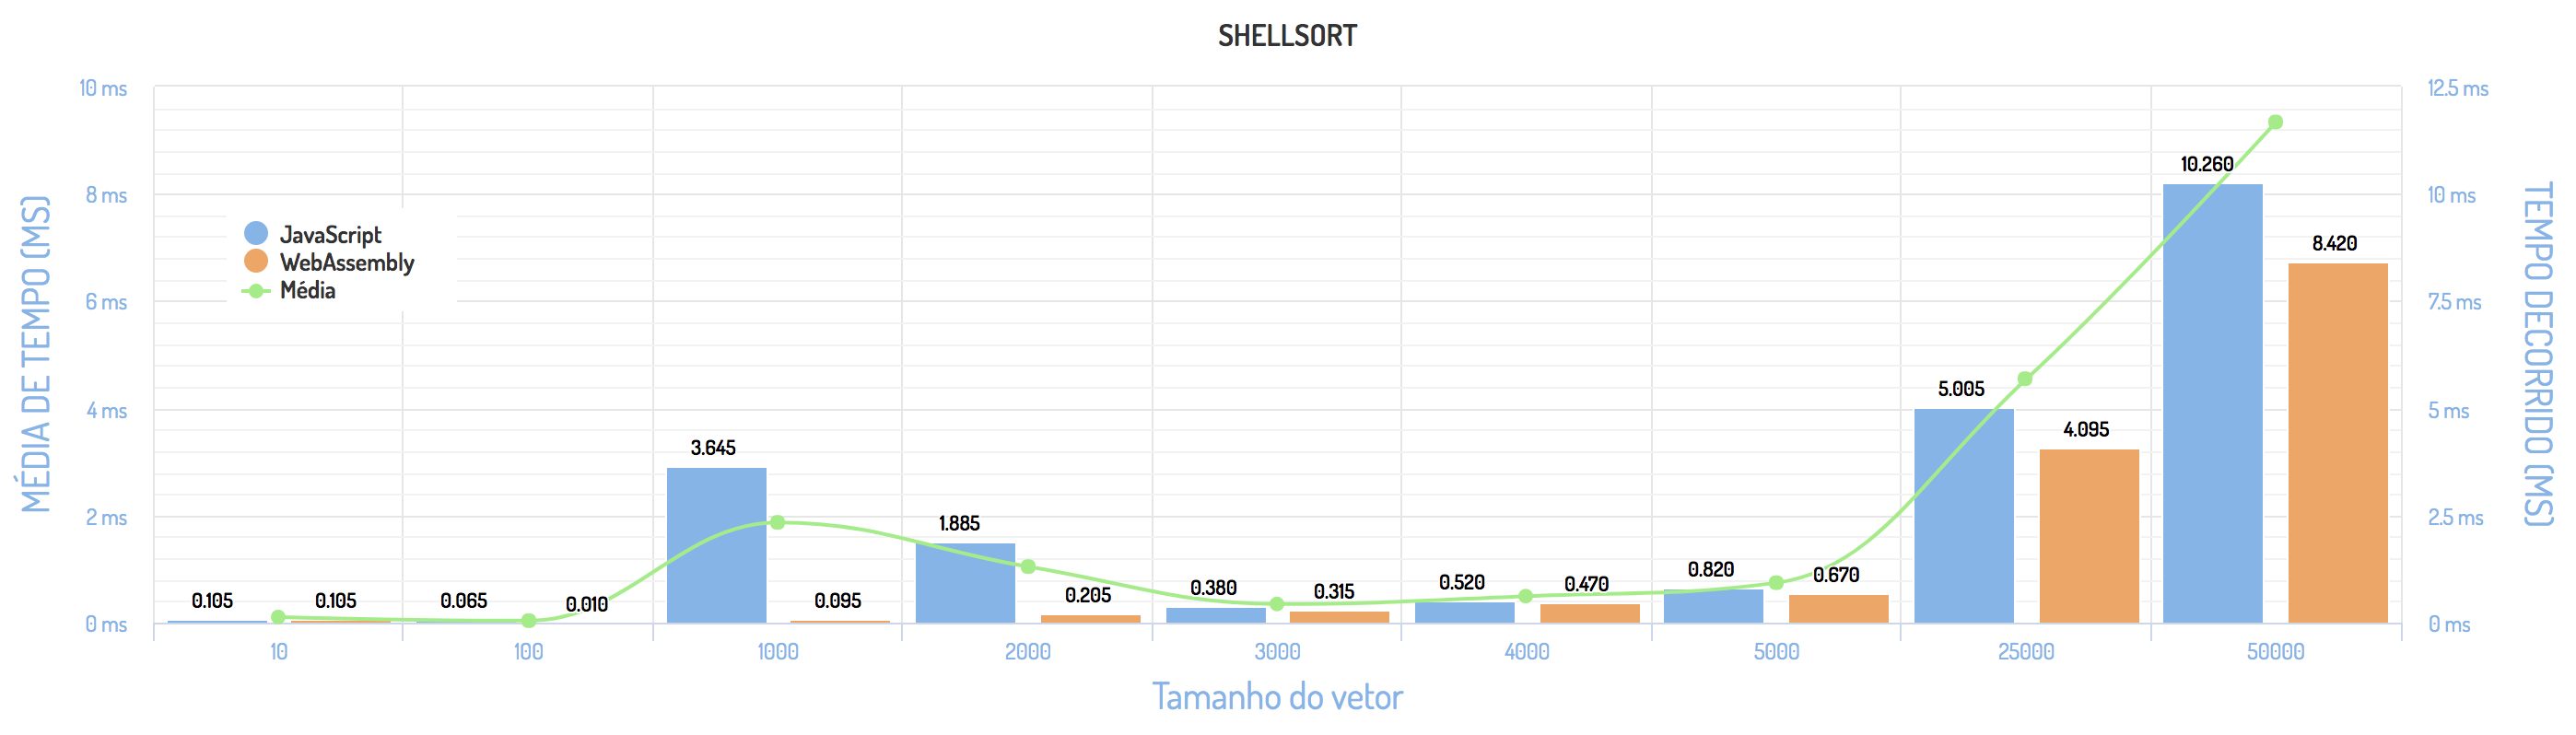
\includegraphics[width=16cm]{graphics/shell_sort}}
    }{
    \Fonte{Elaborada pelo autor.}
    }
\end{figure}

\begin{figure}[h!]
    \centering
    \Caption{\label{fig:image-12} Resultados do algoritmo \textit{QuickSort}}
    \UECEfig{}{
    \fbox{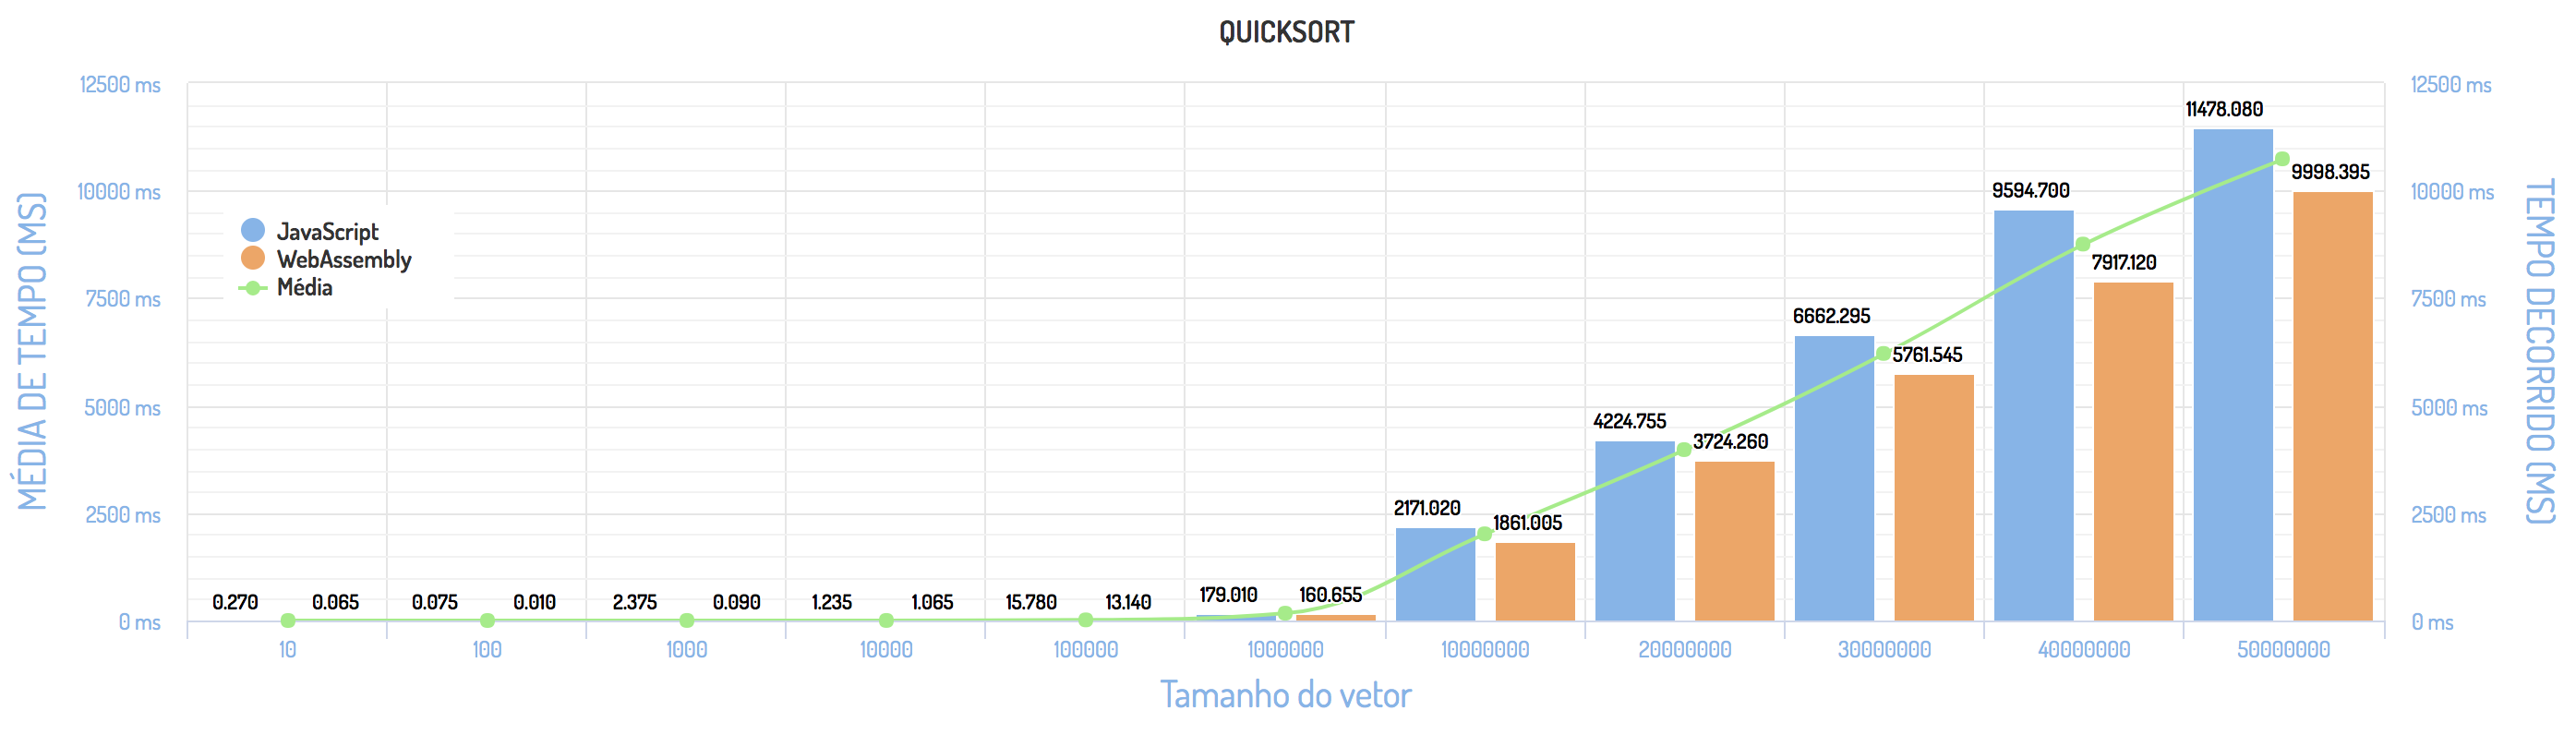
\includegraphics[width=16cm]{graphics/quick_sort}}
    }{
    \Fonte{Elaborada pelo autor.}
    }
\end{figure}

Com base nos resultados exibidos nas figuras \ref{fig:image-10}, \ref{fig:image-11} e
\ref{fig:image-12}, pode-se observar que em quase todos os casos, os algoritmos escritos
em \textit{WebAssembly} tiveram performance superior aos escritos em \textit{JavaScript},
com apenas duas exceções: a primeira, na execução do algoritmo que busca o n-ésimo termo
da sequência \textit{Fibonacci}, em que a implementação escrita em \textit{WebAssembly}
obteve resultado inferior a implementação escrita em \textit{JavaScript}; e a segunda
exceção, obtida na implementação do algoritmo \textit{ShellSort}, em que o algoritmo
escrito em \textit{WebAssembly} obteve aproximadamente o mesmo tempo de execução que o
algoritmo escrito em \textit{JavaScript}.

Em cada algoritmo testado, houveram execuções que apresentaram disparidade bastante
significativa:

\begin{itemize}
    \item \textbf{N-ésimo termo da sequência \textit{Fibonacci}}: na busca pelo vigésimo
    termo da sequência, o tempo utilizado pelo algoritmo escrito em \textit{JavaScript}
    foi de aproximadamente 2300\% superior ao utilizado pelo algoritmo escrito em
    \textit{WebAssembly}.
    \item \textbf{\textit{ShellSort}}: na execução que utilizou um vetor com 1000
    elementos, o tempo utilizado pelo algoritmo escrito em \textit{JavaScript} foi de
    aproximadamente 3700\% superior ao utilizado pelo algoritmo escrito em
    \textit{WebAssembly}.
    \item \textbf{\textit{QuickSort}}: na execução que utilizou um vetor com 1000
    elementos, o tempo utilizado pelo algoritmo escrito em \textit{JavaScript} foi de
    aproximadamente 2500\% superior ao utilizado pelo algoritmo escrito em
    \textit{WebAssembly}.
\end{itemize}

\section{Discussão}
\label{ssec:discussion}

De acordo com o que foi apresentado na seção anterior, é possível perceber que o
desempenho de um algoritmo escrito em \textit{WebAssembly} é na maioria dos casos,
superior ao mesmo algoritmo escrito em \textit{JavaScript}. Isso é devido a sua execução,
enquanto um código escrito em \textit{JavaScript} precisa ser transformado em uma Árvore
de Sintaxe Abstrata e posteriormente convertido em uma representação intermediária, um
código escrito em \textit{WebAssembly} não precisa realizar esses passos, pois ele já é
uma representação intermediária, precisando apenas ser decodificado e verificado para
garantir que não há erros em sua estrutura interna.

Um código escrito em \textit{JavaScript} é compilado durante sua execução, utilizando o
compilador \textit{Just-in-Time}, e dependendo dos tipos que são utilizados em tempo de
execução, múltiplas versões do mesmo código precisam ser compilados utilizando o
compilador de otimização, para garantir que um bloco de código será otimizado
independente dos tipos de dados utilizados internamente, e isso possui um custo elevado
devido ter que monitorar os tipos de dados em execução. Outra observação importante é que
os compiladores JIT precisam gerenciar a relação custo-benefício entre tempos de
carregamento mais rápidos e tempos de execução mais rápidos. Se for gasto mais tempo
compilando e otimizando com antecedência, isso irá acelerar a execução do código, mas irá
deixar a inicialização desse mesmo bloco de código mais lento.

Um fator importante a ser notado sobre \textit{WebAssembly}, é que ele já possui uma
representação intermediária mais próxima do código de máquina, o que acelera sua execução
devido ter que fazer traduções menos complexas de instruções. Outro ponto é que os tipos
de dados fazem parte do algoritmo, o que permite novas abordagens, como por exemplo
paralelizar o trabalho de compilação e execução.

O tempo de carregamento de um arquivo \textit{WebAssembly} também é inferior ao de um
arquivo \textit{JavaScript}, pois possui uma representação binária desenvolvida para ser
mais compacta. Além disso, atualizações mais recentes nos motores \textit{JavaScript}
permitem iniciar o processo de compilação enquanto os \textit{bytes} do arquivo ainda
estão sendo recebidos pelo navegador.
    \chapter{Conclusão}
\label{chap:conclusion}

\section{Considerações finais}
\label{ssec:final-considerations}

Este trabalho se dispôs a fazer uma análise de uma tecnologia emergente no mercado,
chamada de \textit{WebAssembly}, que tem como principal objetivo permitir que aplicações
de alto desempenho sejam executados na \textit{web}, porém não faz quaisquer pressupostos
específicos da \textit{web} ou requer quaisquer recursos específicos da \textit{web},
sendo assim pode ser empregado em outros ambientes.

Com base no que foi apresentado neste trabalho, pode-se observar que \textit{WebAssembly}
se destaca em relação a performance devido alguns aspectos diretamente ligados a seus
objetivos de projeto. Um ponto a ser destacado em relação a \textit{WebAssembly}, é que o
mesmo possui uma representação intermediária binária extremamente compacta, o que faz com
que sua transmissão seja mais eficiente que um arquivo textual comum, como por exemplo um
arquivo \textit{JavaScript}. Além disso, cada arquivo binário representa um único módulo
e é dividido em seções, e cada seção é dividida em funções. Isso significa que a latência
de carregamento de um arquivo pode ser minimizada, ao iniciar o processo de compilação a
medida em que as funções desse arquivo estão sendo recebidas. Junto com essa abordagem,
é possível paralelizar o processo de compilação, distribuindo o processamento dessas
funções, assim como é feito pelos motores \textit{V8} e \textit{SpiderMonkey}.

Foi analisado neste trabalho, por meio de experimentos, que a execução de um código
escrito em \textit{WebAssembly} possui performance superior a um código escrito em
\textit{JavaScript} na maioria dos casos, através da execução dos algoritmos:
\textit{ShellSort}, \textit{QuickSort} e o algoritmo que busca o n-ésimo termo da
sequência \textit{Fibonacci}. O motivo dessa eficiência pode ser compreendida devido
diferenças cruciais entre sua execução e a execução de um algoritmo escrito em
\textit{JavaScript}. Uma diferença importante entre um algoritmo escrito em
\textit{WebAssembly} e \textit{JavaScript}, é que enquanto um algoritmo em
\textit{JavaScript} precisa ser analisado, para posteriormente ser gerada a Árvore de
Sintaxe Abstrata e em seguida a representação intermediária, para só então possa ser
convertido em código de máquina, um algoritmo em \textit{WebAssembly} já é uma
representação intermediária, e ainda mais eficiente que a representação gerada para um
código \textit{JavaScript} em alguns motores, precisando apenas ser convertido em código
de máquina.

\section{Trabalhos futuros}
\label{ssec:future-works}

Como continuação deste trabalho, deseja-se obter mais métricas de desempenho na execução
de cada algoritmo, de forma que se consiga realizar uma análise mais precisa sobre
diferenças de performance entre \textit{WebAssembly} e \textit{JavaScript}. Além disso,
estabelecer uma metodologia de análise de desempenho voltada a \textit{WebAssembly},
através de uma biblioteca criada com esse propósito, em que seja possível informar as
funções a serem testadas e as regras dos dados de entrada e essa biblioteca execute as
funções passando os dados corretos obedecendo as regras estabelecidas e gere todas as
métricas obtidas com base na execução de cada função isoladamente.


\glsaddall

    %Elementos pós-textuais
    \bibliography{elements/pos-textual/referencias}
    \imprimirglossario
    \imprimirindice

\end{document}